% ====================================================================================
\chapter{Transformer实战：显存、算力与工程实现}
% ====================================================================================

\section*{引言：从论文到实验室}

\marginnote{本章内容是你在实验室跑实验必须具备的"工程直觉"。不懂这些，代码写对了也跑不起来。}

在前面的章节中，我们深入理解了Transformer的数学原理。但当你真正要在实验室训练或部署模型时，会遇到一系列非常实际的问题：

\begin{itemize}
    \item "导师给了我一个7B的模型，实验室的显卡能跑吗？"
    \item "为什么我的训练刚开始就报OOM（Out of Memory）？"
    \item "同学说他用4张卡，我只有2张，我的实验要跑多久？"
\end{itemize}

这些问题的答案需要你具备\textbf{工程直觉}——能够快速估算显存、预测训练时间、写出正确的代码。

本章分为四个部分：
\begin{enumerate}
    \item \textbf{硬件基础}：了解你手里的GPU能做什么
    \item \textbf{显存估算}：判断实验能不能跑起来
    \item \textbf{吞吐量计算}：预估实验要跑多久
    \item \textbf{代码实现}：手写核心组件
\end{enumerate}

% ====================================================================================
\section{认识你的GPU}
% ====================================================================================

\marginnote{\textbf{黄仁勋与NVIDIA}：NVIDIA创始人黄仁勋(Jensen Huang)是AI计算革命的关键人物。2006年推出CUDA让GPU可编程，2012年AlexNet用GPU训练催生深度学习浪潮，如今NVIDIA市值超2万亿美元。深度学习的成功很大程度上归功于GPU的并行计算能力。}

% ------------------------------------------------------------------------------------
\subsection{常见GPU参数速查}
% ------------------------------------------------------------------------------------

作为学生，你可能接触到以下几类GPU：

\begin{table}[h]
\centering
\small
\renewcommand{\arraystretch}{1.3}
\begin{tabular}{l|c|c|c|c|c}
\toprule
\textbf{型号} & \textbf{显存} & \textbf{FP16算力} & \textbf{显存带宽} & \textbf{功耗} & \textbf{定位} \\
\midrule
\multicolumn{6}{c}{\textit{消费级（个人/小实验室常见）}} \\
\midrule
RTX 3080 & 10 GB & 30 TFLOPS & 760 GB/s & 320W & 入门深度学习 \\
RTX 3090 & 24 GB & 36 TFLOPS & 936 GB/s & 350W & 个人炼丹主力 \\
RTX 4080 & 16 GB & 49 TFLOPS & 717 GB/s & 320W & 性价比之选 \\
RTX 4090 & 24 GB & 83 TFLOPS & 1008 GB/s & 450W & 消费级天花板 \\
\midrule
\multicolumn{6}{c}{\textit{专业级（实验室/计算中心常见）}} \\
\midrule
A100 40GB & 40 GB & 312 TFLOPS & 1555 GB/s & 400W & 主流科研卡 \\
A100 80GB & 80 GB & 312 TFLOPS & 2039 GB/s & 400W & 大模型训练 \\
H100 SXM & 80 GB & 990 TFLOPS & 3350 GB/s & 700W & 最新旗舰 \\
\midrule
\multicolumn{6}{c}{\textit{国产替代（部分高校可能接触）}} \\
\midrule
华为910B & 64 GB & 320 TFLOPS & 1200 GB/s & 400W & 国产主力 \\
\bottomrule
\end{tabular}
\caption{常见GPU参数对比（FP16/BF16算力，2024年数据）}
\end{table}

\marginnote{\textbf{TFLOPS}：每秒万亿次浮点运算。1 TFLOPS = $10^{12}$ FLOPS。这是衡量GPU计算能力的核心指标。}

\paragraph{几个关键概念}

\begin{itemize}
    \item \textbf{显存（VRAM）}：GPU的"内存"，决定能装多大的模型
    \item \textbf{算力（FLOPS）}：计算速度，决定训练/推理多快
    \item \textbf{显存带宽}：数据搬运速度，大模型推理的瓶颈往往在这里
    \item \textbf{功耗}：电费和散热的考量，实验室可能有限制
\end{itemize}

% ------------------------------------------------------------------------------------
\subsection{数据精度与存储}
% ------------------------------------------------------------------------------------

不同的数值精度决定了模型占用的显存大小：

\begin{table}[h]
\centering
\renewcommand{\arraystretch}{1.3}
\begin{tabular}{l|c|c|c|l}
\toprule
\textbf{精度} & \textbf{位数} & \textbf{字节} & \textbf{数值范围} & \textbf{典型用途} \\
\midrule
FP32 & 32 bit & 4 B & $\pm 3.4 \times 10^{38}$ & 传统训练、优化器状态 \\
TF32 & 19 bit & 4 B & 同FP32 & A100默认训练精度 \\
FP16 & 16 bit & 2 B & $\pm 6.5 \times 10^{4}$ & 混合精度训练 \\
BF16 & 16 bit & 2 B & $\pm 3.4 \times 10^{38}$ & 大模型训练（推荐） \\
INT8 & 8 bit & 1 B & $-128 \sim 127$ & 量化推理 \\
INT4 & 4 bit & 0.5 B & $-8 \sim 7$ & 激进量化 \\
\bottomrule
\end{tabular}
\caption{常见数值精度对比}
\end{table}

\begin{figure}[h]
\centering
\begin{tikzpicture}[scale=0.9]
    % FP32
    \node[font=\bfseries] at (-2, 2) {FP32:};
    \draw (0, 1.7) rectangle (0.8, 2.3);
    \node[font=\scriptsize] at (0.4, 2) {符号};
    \draw (0.8, 1.7) rectangle (3.2, 2.3);
    \node[font=\scriptsize] at (2, 2) {指数 (8位)};
    \draw (3.2, 1.7) rectangle (8, 2.3);
    \node[font=\scriptsize] at (5.6, 2) {尾数 (23位)};
    
    % FP16
    \node[font=\bfseries] at (-2, 1) {FP16:};
    \draw (0, 0.7) rectangle (0.5, 1.3);
    \node[font=\scriptsize] at (0.25, 1) {符};
    \draw (0.5, 0.7) rectangle (2, 1.3);
    \node[font=\scriptsize] at (1.25, 1) {指数 (5位)};
    \draw (2, 0.7) rectangle (5, 1.3);
    \node[font=\scriptsize] at (3.5, 1) {尾数 (10位)};
    
    % BF16
    \node[font=\bfseries] at (-2, 0) {BF16:};
    \draw (0, -0.3) rectangle (0.5, 0.3);
    \node[font=\scriptsize] at (0.25, 0) {符};
    \draw (0.5, -0.3) rectangle (2.9, 0.3);
    \node[font=\scriptsize] at (1.7, 0) {指数 (8位)};
    \draw (2.9, -0.3) rectangle (5, 0.3);
    \node[font=\scriptsize] at (3.95, 0) {尾数 (7位)};
    
    % 说明
    \node[right, font=\small, gray] at (8.5, 2) {精度最高，但慢且费显存};
    \node[right, font=\small, gray] at (5.5, 1) {容易溢出（范围小）};
    \node[right, font=\small, gray] at (5.5, 0) {范围大，精度够用（推荐）};
\end{tikzpicture}
\caption{不同浮点格式的位分配}
\end{figure}

\begin{keyidea}[BF16 vs FP16]
\begin{itemize}
    \item \textbf{FP16}：尾数多（精度高），但指数少（范围小），训练时容易溢出
    \item \textbf{BF16}：指数与FP32相同（范围大），尾数少但够用，训练更稳定
    \item \textbf{实践建议}：如果你的GPU支持BF16（A100、H100、RTX 30/40系列），优先用BF16
\end{itemize}
\end{keyidea}

% ====================================================================================
\section{显存估算：你的实验能跑吗？}
% ====================================================================================

显存是深度学习的"硬通货"。显存不够，代码写得再对也跑不起来。

% ------------------------------------------------------------------------------------
\subsection{模型参数的显存占用}
% ------------------------------------------------------------------------------------

\begin{keyformula}[title=模型显存速算]
\begin{equation}
    \text{模型显存 (GB)} = \text{参数量 (B)} \times \text{每参数字节数}
\end{equation}

速算口诀：
\begin{itemize}
    \item FP32：参数量 $\times$ 4
    \item FP16/BF16：参数量 $\times$ 2
    \item INT8：参数量 $\times$ 1
    \item INT4：参数量 $\times$ 0.5
\end{itemize}
\end{keyformula}

\begin{table}[h]
\centering
\renewcommand{\arraystretch}{1.3}
\begin{tabular}{l|c|c|c|c|c}
\toprule
\textbf{模型} & \textbf{参数量} & \textbf{FP32} & \textbf{FP16/BF16} & \textbf{INT8} & \textbf{INT4} \\
\midrule
GPT-2 & 1.5B & 6 GB & 3 GB & 1.5 GB & 0.75 GB \\
LLaMA-7B & 7B & 28 GB & 14 GB & 7 GB & 3.5 GB \\
LLaMA-13B & 13B & 52 GB & 26 GB & 13 GB & 6.5 GB \\
Qwen-14B & 14B & 56 GB & 28 GB & 14 GB & 7 GB \\
LLaMA-70B & 70B & 280 GB & 140 GB & 70 GB & 35 GB \\
\bottomrule
\end{tabular}
\caption{常见模型的参数显存需求（仅模型权重）}
\end{table}

\begin{example}[判断能否跑LLaMA-7B推理]
\textbf{场景}：实验室有一张RTX 3090（24GB），想跑LLaMA-7B推理。

\textbf{分析}：
\begin{itemize}
    \item FP16加载：$7 \times 2 = 14$ GB $\checkmark$ 可以
    \item 还剩 $24 - 14 = 10$ GB 给KV Cache和其他开销
    \item 结论：\textbf{可以跑}，但长文本生成时KV Cache可能爆显存
\end{itemize}

\textbf{如果只有RTX 3080（10GB）}：
\begin{itemize}
    \item FP16加载：14 GB > 10 GB $\times$ 跑不了
    \item INT4量化：$7 \times 0.5 = 3.5$ GB $\checkmark$ 可以
    \item 结论：必须用\textbf{4-bit量化}（如GPTQ、AWQ）
\end{itemize}
\end{example}

% ------------------------------------------------------------------------------------
\subsection{训练显存：为什么比推理大这么多？}
% ------------------------------------------------------------------------------------

新手常见困惑：为什么推理只要14GB，训练却要上百GB？

答案：训练需要存储的东西远不止模型权重。

\begin{figure}[h]
\centering
\begin{tikzpicture}[>=stealth, scale=0.85]
    % 推理
    \begin{scope}[xshift=-4.5cm]
        \node[font=\bfseries] at (1, 5.5) {推理};
        
        \draw[fill=blue!30] (0, 0) rectangle (2, 3);
        \node at (1, 1.5) {模型权重};
        \node[font=\small] at (1, 0.8) {14 GB};
        
        \draw[fill=gray!20] (0, 3) rectangle (2, 4);
        \node[font=\small] at (1, 3.5) {KV Cache};
        
        \draw[<->] (2.5, 0) -- (2.5, 4);
        \node[right, font=\small] at (2.5, 2) {$\approx$16 GB};
    \end{scope}
    
    % 训练
    \begin{scope}[xshift=3cm]
        \node[font=\bfseries] at (1.5, 5.5) {全量微调};
        
        \draw[fill=blue!30] (0, 0) rectangle (3, 1.5);
        \node at (1.5, 0.75) {模型权重 (FP16)};
        \node[font=\small, gray] at (1.5, 0.3) {14 GB};
        
        \draw[fill=green!30] (0, 1.5) rectangle (3, 3);
        \node at (1.5, 2.25) {梯度 (FP16)};
        \node[font=\small, gray] at (1.5, 1.8) {14 GB};
        
        \draw[fill=orange!30] (0, 3) rectangle (3, 6);
        \node at (1.5, 4.5) {优化器状态};
        \node[font=\small] at (1.5, 4) {(Adam, FP32)};
        \node[font=\small, gray] at (1.5, 3.5) {56 GB};
        
        \draw[fill=red!20] (0, 6) rectangle (3, 7.5);
        \node at (1.5, 6.75) {激活值};
        \node[font=\small, gray] at (1.5, 6.3) {可变};
        
        \draw[<->] (3.5, 0) -- (3.5, 6);
        \node[right, font=\small] at (3.5, 3) {$\geq$84 GB};
        \node[right, font=\scriptsize, red] at (3.5, 2.3) {一张A100都不够！};
    \end{scope}
\end{tikzpicture}
\caption{LLaMA-7B推理 vs 训练的显存对比}
\end{figure}

\paragraph{训练显存的四个组成部分}

\begin{enumerate}
    \item \textbf{模型权重}：和推理一样
    \begin{equation}
        M_{\text{weights}} = N \times \text{dtype\_size}
    \end{equation}
    
    \item \textbf{梯度}：每个参数对应一个梯度，大小与权重相同
    \begin{equation}
        M_{\text{gradients}} = N \times \text{dtype\_size}
    \end{equation}
    
    \item \textbf{优化器状态}：这是大头！以Adam为例：
    \begin{itemize}
        \item 一阶矩（Momentum）：$m_t = \beta_1 m_{t-1} + (1-\beta_1) g_t$
        \item 二阶矩（Variance）：$v_t = \beta_2 v_{t-1} + (1-\beta_2) g_t^2$
        \item 通常用FP32存储以保证数值稳定
    \end{itemize}
    \begin{equation}
        M_{\text{optimizer}} = N \times 2 \times 4 = 8N \quad \text{(Adam)}
    \end{equation}
    
    \item \textbf{激活值}：前向传播的中间结果，反向时要用
    \begin{itemize}
        \item 取决于Batch Size、序列长度、模型深度
        \item 可以用\textbf{梯度检查点}节省（用计算换显存）
    \end{itemize}
\end{enumerate}

\begin{keyformula}[title=全量微调显存估算]
\begin{equation}
    M_{\text{train}} \approx \underbrace{2N}_{\text{权重}} + \underbrace{2N}_{\text{梯度}} + \underbrace{8N}_{\text{优化器}} + M_{\text{激活}} = 12N + M_{\text{激活}}
\end{equation}

简化记忆：\textbf{训练显存 $\approx$ 推理显存 $\times$ 6倍}（不含激活值）
\end{keyformula}

\begin{table}[h]
\centering
\renewcommand{\arraystretch}{1.3}
\begin{tabular}{l|c|c|c|c}
\toprule
\textbf{模型} & \textbf{FP16推理} & \textbf{全量微调} & \textbf{单卡可行性} & \textbf{解决方案} \\
\midrule
GPT-2 (1.5B) & 3 GB & $\approx$20 GB & RTX 3090 ✓ & 单卡可跑 \\
LLaMA-7B & 14 GB & $\approx$100 GB & A100-80G ✗ & DeepSpeed / LoRA \\
LLaMA-13B & 26 GB & $\approx$180 GB & 单卡不可能 & 多卡并行 \\
LLaMA-70B & 140 GB & $\approx$1 TB & 单卡不可能 & 集群训练 \\
\bottomrule
\end{tabular}
\caption{不同模型的训练显存需求与可行性}
\end{table}

% ------------------------------------------------------------------------------------
\subsection{KV Cache：长文本的显存杀手}
% ------------------------------------------------------------------------------------

自回归生成时，为避免重复计算，需要缓存历史token的Key和Value。

\begin{keyformula}[title=KV Cache显存]
\begin{equation}
    M_{KV} = 2 \times L \times S \times H \times D_{\text{type}}
\end{equation}
\begin{itemize}
    \item 2：K和V各一份
    \item $L$：Transformer层数
    \item $S$：序列长度（输入 + 已生成）
    \item $H$：隐藏层维度
    \item $D_{\text{type}}$：每元素字节数（FP16为2）
\end{itemize}
\end{keyformula}

\begin{example}[KV Cache计算]
\textbf{配置}：LLaMA-7B（32层，$H=4096$），序列长度4K，Batch=1，FP16

\begin{align}
    M_{KV} &= 2 \times 32 \times 4096 \times 4096 \times 2 \text{ Bytes} \\
    &= 2,147,483,648 \text{ Bytes} \approx 2 \text{ GB}
\end{align}

\textbf{追问}：如果Batch Size变成16呢？
\begin{equation}
    M_{KV} = 2 \text{ GB} \times 16 = 32 \text{ GB}
\end{equation}

这就是为什么大Batch + 长序列推理这么吃显存。
\end{example}

\begin{table}[h]
\centering
\small
\renewcommand{\arraystretch}{1.3}
\begin{tabular}{l|c|c|c|c}
\toprule
\textbf{序列长度} & \textbf{Batch=1} & \textbf{Batch=8} & \textbf{Batch=32} & \textbf{Batch=64} \\
\midrule
2K & 0.5 GB & 4 GB & 16 GB & 32 GB \\
4K & 1 GB & 8 GB & 32 GB & 64 GB \\
8K & 2 GB & 16 GB & 64 GB & 128 GB \\
32K & 8 GB & 64 GB & 256 GB & 512 GB \\
128K & 32 GB & 256 GB & 1 TB & 2 TB \\
\bottomrule
\end{tabular}
\caption{LLaMA-7B的KV Cache显存（FP16）}
\end{table}

\paragraph{缓解KV Cache的方法}

\begin{itemize}
    \item \textbf{KV Cache量化}：用INT8存储K和V，显存减半
    \item \textbf{GQA}（Grouped Query Attention）：多个Query头共享K/V，LLaMA-2/3已采用
    \item \textbf{PagedAttention}：动态分配KV Cache，vLLM使用的技术
    \item \textbf{滑动窗口}：只保留最近的K/V，Mistral采用
\end{itemize}

% ------------------------------------------------------------------------------------
\subsection{显存速查表}
% ------------------------------------------------------------------------------------

\begin{table}[h]
\centering
\small
\renewcommand{\arraystretch}{1.4}
\begin{tabular}{l|l|l}
\toprule
\textbf{场景} & \textbf{速算公式} & \textbf{7B模型示例} \\
\midrule
FP16推理 & $2 \times N$ & $2 \times 7 = 14$ GB \\
FP32推理 & $4 \times N$ & $4 \times 7 = 28$ GB \\
INT8推理 & $1 \times N$ & $1 \times 7 = 7$ GB \\
INT4推理 & $0.5 \times N$ & $0.5 \times 7 = 3.5$ GB \\
\midrule
全量微调 & $\approx 12 \times N$ & $12 \times 7 = 84$ GB \\
LoRA微调 & $\approx 2 \times N$ & $\approx 16$ GB \\
\midrule
KV Cache (FP16) & $4 \times L \times S \times H$ & 见上表 \\
\bottomrule
\end{tabular}
\caption{显存估算速查表（$N$单位：B参数，结果单位：GB）}
\end{table}

% ====================================================================================
\section{吞吐量计算：实验要跑多久？}
% ====================================================================================

显存够了之后，下一个问题是：\textbf{实验要跑多久？}

% ------------------------------------------------------------------------------------
\subsection{计算量估算}
% ------------------------------------------------------------------------------------

\paragraph{Transformer的计算量}

对于一个Transformer模型，前向传播的计算量约为：

\begin{keyformula}[title=Transformer计算量估算]
\begin{equation}
    \text{FLOPs}_{\text{forward}} \approx 2 \times N \times S
\end{equation}
其中 $N$ 是参数量，$S$ 是序列长度。

训练时还需要反向传播（约等于2倍前向），所以：
\begin{equation}
    \text{FLOPs}_{\text{train}} \approx 6 \times N \times S \quad \text{(每个token)}
\end{equation}
\end{keyformula}

\marginnote{这个公式假设模型以矩阵乘法为主，忽略了激活函数等开销。实际计算量可能略高。}

\begin{example}[训练计算量估算]
\textbf{任务}：用100B tokens预训练一个7B模型

\textbf{计算}：
\begin{align}
    \text{总FLOPs} &= 6 \times 7 \times 10^9 \times 100 \times 10^9 \\
    &= 4.2 \times 10^{21} \text{ FLOPs} \\
    &= 4.2 \text{ ZFLOPs}
\end{align}
\end{example}

% ------------------------------------------------------------------------------------
\subsection{训练时间估算}
% ------------------------------------------------------------------------------------

知道计算量后，可以估算训练时间：

\begin{keyformula}[title=训练时间估算]
\begin{equation}
    T = \frac{\text{总FLOPs}}{\text{GPU数量} \times \text{单卡算力} \times \text{利用率}}
\end{equation}
\end{keyformula}

\paragraph{GPU利用率（MFU）}

实际训练中，GPU不可能100\%满载。\textbf{模型算力利用率}（Model FLOPS Utilization, MFU）通常在30\%-60\%：

\begin{table}[h]
\centering
\renewcommand{\arraystretch}{1.3}
\begin{tabular}{l|c|l}
\toprule
\textbf{场景} & \textbf{典型MFU} & \textbf{原因} \\
\midrule
单卡训练小模型 & 40-50\% & 数据加载、小batch效率低 \\
单卡训练大模型 & 50-60\% & batch大，计算密集 \\
多卡数据并行 & 40-55\% & 通信开销 \\
多卡模型并行 & 30-45\% & 流水线气泡、通信开销 \\
\bottomrule
\end{tabular}
\caption{不同场景的典型GPU利用率}
\end{table}

\begin{example}[预训练时间估算]
\textbf{任务}：用100B tokens预训练7B模型

\textbf{配置}：8张A100-80GB，MFU假设50\%

\textbf{计算}：
\begin{align}
    \text{有效算力} &= 8 \times 312 \text{ TFLOPS} \times 50\% = 1248 \text{ TFLOPS} \\
    T &= \frac{4.2 \times 10^{21}}{1248 \times 10^{12}} = 3.37 \times 10^{6} \text{ 秒} \\
    &\approx 39 \text{ 天}
\end{align}

\textbf{如果用64张H100}：
\begin{align}
    \text{有效算力} &= 64 \times 990 \text{ TFLOPS} \times 50\% = 31680 \text{ TFLOPS} \\
    T &= \frac{4.2 \times 10^{21}}{31680 \times 10^{12}} \approx 1.5 \text{ 天}
\end{align}
\end{example}

% ------------------------------------------------------------------------------------
\subsection{不同规模的训练成本参考}
% ------------------------------------------------------------------------------------

\begin{table}[h]
\centering
\small
\renewcommand{\arraystretch}{1.4}
\begin{tabular}{l|c|c|c|c}
\toprule
\textbf{模型} & \textbf{训练数据} & \textbf{总FLOPs} & \textbf{8×A100时间} & \textbf{64×H100时间} \\
\midrule
GPT-2 (1.5B) & 40B tokens & $3.6 \times 10^{20}$ & 3天 & 4小时 \\
LLaMA-7B & 1T tokens & $4.2 \times 10^{22}$ & 1年+ & 42天 \\
LLaMA-13B & 1T tokens & $7.8 \times 10^{22}$ & 2年+ & 78天 \\
LLaMA-70B & 1.4T tokens & $5.9 \times 10^{23}$ & 15年+ & 1.5年 \\
\bottomrule
\end{tabular}
\caption{预训练时间估算（MFU=50\%）}
\end{table}

\begin{remark}
从这个表可以看出：
\begin{itemize}
    \item 预训练大模型需要\textbf{大量算力}，不是学生个人能承担的
    \item 学生能做的是\textbf{微调}（只需要原训练的千分之一算力）
    \item 或者\textbf{小模型实验}（验证想法后再申请资源）
\end{itemize}
\end{remark}

% ------------------------------------------------------------------------------------
\subsection{微调时间估算}
% ------------------------------------------------------------------------------------

微调比预训练快得多，因为数据量小：

\begin{example}[LoRA微调时间估算]
\textbf{任务}：对LLaMA-7B做LoRA微调，10K条指令数据，平均长度512 tokens

\textbf{计算}：
\begin{align}
    \text{总tokens} &= 10000 \times 512 = 5.12 \times 10^6 \\
    \text{每epoch FLOPs} &= 6 \times 7 \times 10^9 \times 5.12 \times 10^6 = 2.15 \times 10^{17}
\end{align}

\textbf{单张RTX 4090}（83 TFLOPS，MFU 45\%）：
\begin{align}
    \text{每epoch时间} &= \frac{2.15 \times 10^{17}}{83 \times 10^{12} \times 0.45} \approx 5760 \text{ 秒} \approx 1.6 \text{ 小时}
\end{align}

训练3个epoch：\textbf{约5小时}
\end{example}

% ------------------------------------------------------------------------------------
\subsection{推理吞吐量}
% ------------------------------------------------------------------------------------

推理时，我们关心的是\textbf{每秒能生成多少token}（tokens/s）。

\paragraph{推理的两个阶段}

\begin{enumerate}
    \item \textbf{Prefill}（预填充）：处理输入的所有token，计算密集
    \item \textbf{Decode}（解码）：逐个生成输出token，显存带宽受限
\end{enumerate}

\begin{figure}[h]
\centering
\begin{tikzpicture}[>=stealth, scale=0.85]
    % Prefill
    \draw[fill=blue!20] (0, 0) rectangle (3, 2);
    \node at (1.5, 1) {Prefill};
    \node[below, font=\small] at (1.5, 0) {处理输入};
    
    % Decode
    \draw[fill=orange!20] (4, 0) rectangle (10, 2);
    \node at (7, 1) {Decode（自回归生成）};
    \node[below, font=\small] at (7, 0) {逐token生成};
    
    % 时间轴
    \draw[->] (0, -1) -- (11, -1) node[right] {时间};
    
    % 特点标注
    \node[above, font=\small, blue] at (1.5, 2.2) {计算密集};
    \node[above, font=\small, blue] at (1.5, 2.7) {可高度并行};
    
    \node[above, font=\small, orange] at (7, 2.2) {带宽受限};
    \node[above, font=\small, orange] at (7, 2.7) {逐个串行};
\end{tikzpicture}
\caption{推理的两个阶段}
\end{figure}

\paragraph{Decode阶段的吞吐量估算}

Decode阶段是带宽受限的，每生成一个token需要从显存读取整个模型：

\begin{equation}
    \text{最大tokens/s} \approx \frac{\text{显存带宽}}{\text{模型大小}}
\end{equation}

\begin{example}[LLaMA-7B推理吞吐量]
\textbf{配置}：单张A100-80GB（带宽2039 GB/s），FP16

\begin{align}
    \text{理论最大} &= \frac{2039 \text{ GB/s}}{14 \text{ GB}} \approx 145 \text{ tokens/s}
\end{align}

实际由于各种开销，通常能达到\textbf{80-100 tokens/s}。

\textbf{对比RTX 4090}（带宽1008 GB/s）：
\begin{align}
    \text{理论最大} &= \frac{1008}{14} \approx 72 \text{ tokens/s}
\end{align}
实际约\textbf{40-50 tokens/s}。
\end{example}

\begin{table}[h]
\centering
\small
\renewcommand{\arraystretch}{1.3}
\begin{tabular}{l|c|c|c|c}
\toprule
\textbf{GPU} & \textbf{LLaMA-7B} & \textbf{LLaMA-13B} & \textbf{LLaMA-70B} & \textbf{备注} \\
\midrule
RTX 3090 & 30-40 t/s & 需量化 & 不可行 & 消费级 \\
RTX 4090 & 40-50 t/s & 20-25 t/s & 需量化 & 消费级天花板 \\
A100-40GB & 70-90 t/s & 40-50 t/s & 需多卡 & 专业卡 \\
A100-80GB & 80-100 t/s & 50-60 t/s & 15-20 t/s & 大显存 \\
H100 & 150-200 t/s & 100-120 t/s & 40-50 t/s & 最新旗舰 \\
\bottomrule
\end{tabular}
\caption{不同GPU的LLM推理吞吐量参考（FP16，Batch=1，实测范围）}
\end{table}

% ====================================================================================
\section{代码实现：手写Attention}
% ====================================================================================

\marginnote{\textbf{Transformer的诞生}：2017年，Google的Vaswani等人发表``Attention Is All You Need''，用纯注意力机制取代了RNN/CNN，成为现代大模型的基石。论文标题成为深度学习史上最经典的口号之一。}

理解原理后，让我们动手实现核心组件。

% ------------------------------------------------------------------------------------
\subsection{Scaled Dot-Product Attention}
% ------------------------------------------------------------------------------------

\marginnote{\textbf{注意力机制溯源}：注意力机制最早由Bahdanau等人(2014)引入机器翻译，让模型``看向''输入的不同部分。Transformer将其推广为``自注意力''，让序列中的每个位置都能关注其他所有位置。}

回顾公式：
\begin{equation}
    \text{Attention}(Q, K, V) = \text{softmax}\left(\frac{QK^\top}{\sqrt{d_k}}\right) V
\end{equation}

\begin{lstlisting}[language=Python, caption=Scaled Dot-Product Attention]
import torch
import torch.nn.functional as F
import math

def scaled_dot_product_attention(query, key, value, mask=None):
    """
    缩放点积注意力
    
    Args:
        query: [batch, num_heads, seq_len_q, head_dim]
        key:   [batch, num_heads, seq_len_k, head_dim]
        value: [batch, num_heads, seq_len_k, head_dim]
        mask:  [batch, 1, seq_len_q, seq_len_k] 或可广播形状
               1表示保留，0表示遮挡
    
    Returns:
        output: [batch, num_heads, seq_len_q, head_dim]
        attn_weights: [batch, num_heads, seq_len_q, seq_len_k]
    """
    d_k = query.size(-1)  # head_dim
    
    # Step 1: Q @ K^T -> [batch, heads, seq_q, seq_k]
    scores = torch.matmul(query, key.transpose(-2, -1))
    
    # Step 2: 缩放，防止点积过大导致softmax饱和
    scores = scores / math.sqrt(d_k)
    
    # Step 3: 应用mask（可选）
    if mask is not None:
        # mask为0的位置填负无穷，softmax后变成0
        scores = scores.masked_fill(mask == 0, float('-inf'))
    
    # Step 4: softmax归一化（在最后一个维度，即key的位置）
    attn_weights = F.softmax(scores, dim=-1)
    
    # Step 5: 加权求和
    output = torch.matmul(attn_weights, value)
    
    return output, attn_weights
\end{lstlisting}

\begin{example}[运行示例：理解张量维度变化]
让我们用具体数字追踪一次Attention计算：

\begin{lstlisting}[language=Python, caption=Attention维度演示]
# 输入: batch=2, heads=4, seq_len=3, head_dim=8
query = torch.randn(2, 4, 3, 8)
key   = torch.randn(2, 4, 3, 8)
value = torch.randn(2, 4, 3, 8)

output, weights = scaled_dot_product_attention(query, key, value)

print(f"Query shape:   {query.shape}")   # [2, 4, 3, 8]
print(f"Key shape:     {key.shape}")     # [2, 4, 3, 8]
print(f"Scores shape:  {(query @ key.transpose(-2,-1)).shape}")  # [2, 4, 3, 3]
print(f"Weights shape: {weights.shape}") # [2, 4, 3, 3] <- softmax后的注意力权重
print(f"Output shape:  {output.shape}")  # [2, 4, 3, 8]

# 验证：每行注意力权重和为1
print(f"权重和: {weights[0,0,0,:].sum():.4f}")  # 1.0000
\end{lstlisting}

\textbf{矩阵运算追踪}：
\begin{enumerate}
    \item $Q \times K^\top$: $[2,4,3,\mathbf{8}] \times [2,4,\mathbf{8},3] = [2,4,3,3]$ —— 每对位置的相似度
    \item softmax: $[2,4,3,3] \to [2,4,3,3]$ —— 归一化为概率
    \item $\text{weights} \times V$: $[2,4,3,\mathbf{3}] \times [2,4,\mathbf{3},8] = [2,4,3,8]$ —— 加权求和
\end{enumerate}

\textbf{核心洞察}：\textbf{Attention就是三次矩阵乘法}。这正是GPU能高效处理的原因！
\end{example}

\paragraph{关键点解析}

\begin{enumerate}
    \item \textbf{为什么除以$\sqrt{d_k}$？}
    
    假设Q和K的元素独立同分布于$\mathcal{N}(0, 1)$，则点积的方差是$d_k$：
    \begin{equation}
        \text{Var}(q \cdot k) = \sum_{i=1}^{d_k} \text{Var}(q_i k_i) = d_k
    \end{equation}
    
    $d_k$越大，点积值越大，softmax越接近one-hot，梯度越小。缩放后方差为1。
    
    \item \textbf{为什么mask用负无穷？}
    
    因为$\text{softmax}(-\infty) = 0$。如果直接把scores设成0，softmax后不是0而是一个正数。
    
    \item \textbf{softmax在哪个维度？}
    
    \texttt{dim=-1}，即对所有Key位置归一化，保证注意力权重和为1。
\end{enumerate}

% ------------------------------------------------------------------------------------
\subsection{因果掩码（Causal Mask）}
% ------------------------------------------------------------------------------------

自回归生成时，位置$i$只能看到位置$j \leq i$的token：

\begin{lstlisting}[language=Python, caption=生成因果掩码]
def create_causal_mask(seq_len, device='cpu'):
    """
    创建因果掩码（下三角矩阵）
    
    Returns:
        mask: [1, 1, seq_len, seq_len]
    """
    # torch.tril: 下三角矩阵
    mask = torch.tril(torch.ones(seq_len, seq_len, device=device))
    # 扩展维度以便广播到 [batch, heads, seq, seq]
    return mask.unsqueeze(0).unsqueeze(0)

# 示例: seq_len=4
# [[1, 0, 0, 0],
#  [1, 1, 0, 0],
#  [1, 1, 1, 0],
#  [1, 1, 1, 1]]
\end{lstlisting}

\begin{figure}[h]
\centering
\begin{tikzpicture}[scale=0.55]
    % 矩阵格子
    \foreach \i in {0,...,5} {
        \draw[gray] (0, \i) -- (6, \i);
        \draw[gray] (\i, 0) -- (\i, 6);
    }
    \draw[thick] (0, 0) rectangle (6, 6);
    
    % 填充
    \foreach \i in {0,...,5} {
        \foreach \j in {0,...,5} {
            \pgfmathtruncatemacro{\keep}{\j <= \i ? 1 : 0}
            \ifnum\keep=1
                \fill[green!30] (\j, 5-\i) rectangle (\j+1, 6-\i);
                \node[font=\small] at (\j+0.5, 5.5-\i) {1};
            \else
                \fill[red!20] (\j, 5-\i) rectangle (\j+1, 6-\i);
                \node[font=\small] at (\j+0.5, 5.5-\i) {0};
            \fi
        }
    }
    
    % 标签
    \node[above] at (3, 6.3) {Key位置 $j$};
    \node[left, rotate=90] at (-0.5, 3) {Query位置 $i$};
    
    % 说明
    \node[right, font=\small] at (7, 5) {绿色：可以看到};
    \node[right, font=\small] at (7, 4) {红色：不能看到};
    \node[right, font=\small] at (7, 2.5) {位置 $i$ 只能attend到};
    \node[right, font=\small] at (7, 1.8) {位置 $j \leq i$};
\end{tikzpicture}
\caption{因果掩码示例（seq\_len=6）}
\end{figure}

% ------------------------------------------------------------------------------------
\subsection{Multi-Head Attention的维度变换}
% ------------------------------------------------------------------------------------

Multi-Head的关键是正确处理维度：

\begin{equation}
    [B, L, D] \xrightarrow{\text{拆分}} [B, H, L, D_h] \xrightarrow{\text{attention}} [B, H, L, D_h] \xrightarrow{\text{合并}} [B, L, D]
\end{equation}

其中$D = H \times D_h$（总维度 = 头数 $\times$ 每头维度）。

\begin{lstlisting}[language=Python, caption=Multi-Head维度变换]
def split_heads(x, num_heads):
    """
    拆分成多头
    [batch, seq_len, hidden_size] -> [batch, num_heads, seq_len, head_dim]
    """
    batch, seq_len, hidden = x.size()
    head_dim = hidden // num_heads
    
    # reshape: [B, L, H] -> [B, L, num_heads, head_dim]
    x = x.view(batch, seq_len, num_heads, head_dim)
    
    # transpose: [B, L, num_heads, head_dim] -> [B, num_heads, L, head_dim]
    # 把num_heads提前，方便并行计算
    return x.transpose(1, 2)


def merge_heads(x):
    """
    合并多头
    [batch, num_heads, seq_len, head_dim] -> [batch, seq_len, hidden_size]
    """
    batch, num_heads, seq_len, head_dim = x.size()
    
    # transpose回去: [B, num_heads, L, head_dim] -> [B, L, num_heads, head_dim]
    x = x.transpose(1, 2)
    
    # reshape: [B, L, num_heads, head_dim] -> [B, L, hidden]
    # contiguous()保证内存连续，否则view可能报错
    return x.contiguous().view(batch, seq_len, num_heads * head_dim)
\end{lstlisting}

\paragraph{为什么要transpose？}

\texttt{torch.matmul}对最后两个维度做矩阵乘法，前面的维度广播。

把\texttt{num\_heads}放到前面后，每个head的$Q \in \mathbb{R}^{L \times D_h}$和$K \in \mathbb{R}^{L \times D_h}$可以并行相乘。

% ------------------------------------------------------------------------------------
\subsection{完整的Multi-Head Attention}
% ------------------------------------------------------------------------------------

\begin{lstlisting}[language=Python, caption=完整的Multi-Head Attention]
class MultiHeadAttention(nn.Module):
    def __init__(self, hidden_size, num_heads, dropout=0.1):
        super().__init__()
        assert hidden_size % num_heads == 0, "hidden_size必须能被num_heads整除"
        
        self.hidden_size = hidden_size
        self.num_heads = num_heads
        self.head_dim = hidden_size // num_heads
        
        # Q, K, V投影
        self.q_proj = nn.Linear(hidden_size, hidden_size)
        self.k_proj = nn.Linear(hidden_size, hidden_size)
        self.v_proj = nn.Linear(hidden_size, hidden_size)
        
        # 输出投影
        self.out_proj = nn.Linear(hidden_size, hidden_size)
        self.dropout = nn.Dropout(dropout)
        
    def forward(self, x, mask=None):
        """
        自注意力：Q, K, V都来自同一个输入x
        Args:
            x: [batch, seq_len, hidden_size]
            mask: [batch, 1, seq_len, seq_len] 或 None
        """
        batch_size, seq_len, _ = x.size()
        
        # 1. 投影
        Q = self.q_proj(x)  # [B, L, H]
        K = self.k_proj(x)
        V = self.v_proj(x)
        
        # 2. 拆分多头
        Q = self._split_heads(Q)  # [B, num_heads, L, head_dim]
        K = self._split_heads(K)
        V = self._split_heads(V)
        
        # 3. 计算注意力
        scores = torch.matmul(Q, K.transpose(-2, -1)) / math.sqrt(self.head_dim)
        
        if mask is not None:
            scores = scores.masked_fill(mask == 0, float('-inf'))
        
        attn_weights = F.softmax(scores, dim=-1)
        attn_weights = self.dropout(attn_weights)
        
        attn_output = torch.matmul(attn_weights, V)  # [B, num_heads, L, head_dim]
        
        # 4. 合并多头
        attn_output = self._merge_heads(attn_output)  # [B, L, H]
        
        # 5. 输出投影
        output = self.out_proj(attn_output)
        
        return output
    
    def _split_heads(self, x):
        B, L, _ = x.size()
        return x.view(B, L, self.num_heads, self.head_dim).transpose(1, 2)
    
    def _merge_heads(self, x):
        B, _, L, _ = x.size()
        return x.transpose(1, 2).contiguous().view(B, L, self.hidden_size)
\end{lstlisting}

% ====================================================================================
\section{高效微调：LoRA简介}
% ====================================================================================

\marginnote{\textbf{LoRA的诞生}：2021年，微软的Hu等人提出LoRA，让普通研究者也能在消费级显卡上微调大模型。这篇论文引用量已超过5000次，催生了QLoRA、DoRA等一系列变体，成为开源社区微调LLM的标准方法。}

全量微调大模型需要的显存太大。\textbf{LoRA}（Low-Rank Adaptation）是一种参数高效的替代方案。

% ------------------------------------------------------------------------------------
\subsection{核心思想}
% ------------------------------------------------------------------------------------

\begin{keyidea}[title=LoRA的假设]
微调时，权重的更新量$\Delta W$是\textbf{低秩}的。

原来的大矩阵$W \in \mathbb{R}^{d \times d}$可能有1600万参数，但更新量可以用两个小矩阵近似：
\begin{equation}
    \Delta W \approx BA, \quad B \in \mathbb{R}^{d \times r}, \quad A \in \mathbb{R}^{r \times d}
\end{equation}
其中$r$是秩，通常$r = 4, 8, 16$，远小于$d$。
\end{keyidea}

\begin{figure}[h]
\centering
\begin{tikzpicture}[>=stealth, scale=0.8]
    % 原始权重
    \node[draw, rectangle, fill=blue!20, minimum width=2.5cm, minimum height=2.5cm] (W) at (0, 0) {$W$};
    \node[below, font=\small] at (0, -1.5) {$d \times d$};
    \node[below, font=\scriptsize, gray] at (0, -2) {（冻结）};
    
    \node at (2, 0) {$+$};
    
    % B矩阵
    \node[draw, rectangle, fill=green!30, minimum width=0.5cm, minimum height=2.5cm] (B) at (4, 0) {$B$};
    \node[below, font=\small] at (4, -1.5) {$d \times r$};
    
    \node at (5, 0) {$\times$};
    
    % A矩阵
    \node[draw, rectangle, fill=orange!30, minimum width=2.5cm, minimum height=0.5cm] (A) at (7, 0) {$A$};
    \node[below, font=\small] at (7, -0.6) {$r \times d$};
    
    \node at (9.5, 0) {$=$};
    
    % 新权重
    \node[draw, rectangle, fill=purple!20, minimum width=2.5cm, minimum height=2.5cm] (Wnew) at (12, 0) {$W'$};
    \node[below, font=\small] at (12, -1.5) {$d \times d$};
    
    % 标注
    \draw[<->, red, thick] (3.7, -1.25) -- (4.3, -1.25);
    \node[red, below, font=\scriptsize] at (4, -1.4) {很窄!};
\end{tikzpicture}
\caption{LoRA：冻结原权重$W$，只训练低秩矩阵$A$和$B$}
\end{figure}

% ------------------------------------------------------------------------------------
\subsection{参数量与显存}
% ------------------------------------------------------------------------------------

\begin{example}[LoRA参数量计算]
\textbf{设置}：$W$的形状是$[4096, 4096]$，LoRA秩$r=8$

\textbf{计算}：
\begin{align}
    \text{原参数量} &= 4096 \times 4096 = 16,777,216 \approx 16.7\text{M} \\
    \text{LoRA参数} &= 4096 \times 8 + 8 \times 4096 = 65,536 \approx 65\text{K} \\
    \text{比例} &= \frac{65\text{K}}{16.7\text{M}} \approx 0.4\%
\end{align}
\end{example}

LoRA的显存优势：

\begin{itemize}
    \item 原模型\textbf{冻结}：不需要存梯度和优化器状态
    \item 只训练$A$和$B$：参数量小，相应的梯度和优化器状态也小
\end{itemize}

\begin{table}[h]
\centering
\renewcommand{\arraystretch}{1.3}
\begin{tabular}{l|c|c}
\toprule
\textbf{方法} & \textbf{7B模型训练显存} & \textbf{单卡可行性} \\
\midrule
全量微调 & $\approx$100 GB & A100-80GB ✗ \\
LoRA ($r=8$) & $\approx$18 GB & RTX 3090 ✓ \\
QLoRA (4-bit + LoRA) & $\approx$6 GB & RTX 3080 ✓ \\
\bottomrule
\end{tabular}
\caption{不同微调方法的显存需求对比}
\end{table}

% ------------------------------------------------------------------------------------
\subsection{LoRA的关键细节}
% ------------------------------------------------------------------------------------

\paragraph{初始化}

\begin{itemize}
    \item $A$：高斯随机初始化
    \item $B$：\textbf{全零}初始化
\end{itemize}

为什么$B$初始化为0？因为这样初始时$BA = 0$，网络输出与预训练模型完全相同。这保证了微调从一个好的起点开始。

\paragraph{推理时合并权重}

训练完成后，可以把LoRA权重合并到原权重中：

\begin{equation}
    W' = W + BA
\end{equation}

合并后，推理时就是一个普通的线性层，\textbf{没有额外开销}。

\begin{lstlisting}[language=Python, caption=LoRA推理时合并权重]
# 训练完成后
merged_weight = base_weight + lora_B @ lora_A

# 推理时直接用merged_weight，速度与原模型相同
\end{lstlisting}

% ====================================================================================
\section{高效计算：FlashAttention与MoE}
% ====================================================================================

\marginnote{本节介绍两个现代大模型的关键技术：FlashAttention加速注意力计算，MoE降低推理成本。}

% ------------------------------------------------------------------------------------
\subsection{FlashAttention：IO感知的注意力计算}
% ------------------------------------------------------------------------------------

\marginnote{\textbf{FlashAttention}：2022年，斯坦福的Tri Dao在博士期间提出，通过IO感知算法将长序列注意力速度提升2-4倍，并大幅降低显存。该工作发表于NeurIPS 2022，Dao随后创办Together AI公司，FlashAttention已成为几乎所有大模型训练的标配。}

标准注意力计算有一个严重问题：需要存储完整的$N \times N$注意力矩阵。

\begin{keyformula}[title=标准Attention的显存瓶颈]
对于序列长度$N$，标准Attention需要：
\begin{itemize}
    \item 计算：$O(N^2 \cdot d)$ 次浮点运算
    \item 存储：$O(N^2)$ 的注意力矩阵（用于反向传播）
\end{itemize}

当$N = 100K$时，注意力矩阵需要 $100K \times 100K \times 2B = 20$ GB 显存！
\end{keyformula}

FlashAttention的核心思想：\textbf{分块计算 + 重算而非存储}。

\paragraph{算法思路}

\begin{enumerate}
    \item 将$Q, K, V$分成小块（block），每块能装进GPU的高速缓存（SRAM）
    \item 一次只计算一个块的注意力，立即与$V$相乘得到部分输出
    \item 使用在线softmax技巧，边算边累加，无需存储完整的注意力矩阵
    \item 反向传播时，重新计算注意力矩阵（recomputation），用计算换显存
\end{enumerate}

\begin{figure}[h]
\centering
\begin{tikzpicture}[scale=0.8]
    % 左边：标准Attention
    \node[font=\bfseries] at (0, 3.5) {标准Attention};

    % Q, K矩阵
    \draw[fill=blue!20] (0, 0) rectangle (1, 2.5);
    \node at (0.5, 2.8) {\small Q};
    \draw[fill=green!20] (1.5, 0) rectangle (4, 0.8);
    \node at (2.75, 1.1) {\small $K^T$};

    % 大的Attention矩阵
    \draw[fill=red!30] (0, -3) rectangle (2.5, -0.5);
    \node at (1.25, -1.75) {\small Attn};
    \node[font=\scriptsize] at (1.25, -2.3) {$N \times N$};
    \node[font=\scriptsize, red] at (1.25, -3.4) {需要存储！};

    % 箭头
    \draw[->, thick] (2, 0.4) -- (1.25, -0.3);

    % 右边：FlashAttention
    \node[font=\bfseries] at (7, 3.5) {FlashAttention};

    % 分块的Q, K
    \draw[fill=blue!40] (6, 1.8) rectangle (6.8, 2.5);
    \draw[fill=blue!20] (6, 1) rectangle (6.8, 1.7);
    \draw[fill=blue!20] (6, 0.2) rectangle (6.8, 0.9);
    \node at (6.4, 2.8) {\small Q块};

    \draw[fill=green!40] (7.2, 2.2) rectangle (9, 2.5);
    \draw[fill=green!20] (7.2, 1.9) rectangle (9, 2.2);
    \draw[fill=green!20] (7.2, 1.6) rectangle (9, 1.9);
    \node at (8.1, 2.8) {\small $K^T$块};

    % 小的块矩阵
    \draw[fill=orange!40] (6.5, -1.5) rectangle (7.3, -0.7);
    \node[font=\scriptsize] at (6.9, -1.1) {小块};
    \node[font=\scriptsize, green!60!black] at (6.9, -2) {在SRAM中};

    % 输出
    \draw[fill=purple!30] (8, -1.5) rectangle (8.6, -0.7);
    \node[font=\scriptsize] at (8.3, -1.1) {累加};

    % 箭头
    \draw[->, thick] (7.5, 1.6) -- (6.9, -0.5);
    \draw[->, thick] (7.3, -1.1) -- (7.9, -1.1);
\end{tikzpicture}
\caption{FlashAttention通过分块计算避免存储完整注意力矩阵}
\end{figure}

\begin{keyidea}[FlashAttention的核心洞察]
\textbf{GPU的瓶颈不是计算，而是数据搬运}（memory-bound）。

\begin{itemize}
    \item GPU算力：H100有990 TFLOPS
    \item 显存带宽：H100只有3.35 TB/s
    \item 计算/带宽比 = 296 FLOP/Byte，意味着每搬1字节要做296次运算才能喂饱GPU
\end{itemize}

FlashAttention把数据留在高速SRAM中，减少HBM读写，从而同时加速计算和节省显存。
\end{keyidea}

\paragraph{使用方法}

\begin{lstlisting}[language=Python, caption=PyTorch 2.0+ 内置FlashAttention]
import torch.nn.functional as F

# PyTorch 2.0+ 自动使用FlashAttention
output = F.scaled_dot_product_attention(
    query, key, value,
    is_causal=True  # 因果掩码
)

# 手动指定后端
with torch.backends.cuda.sdp_kernel(
    enable_flash=True,
    enable_math=False,
    enable_mem_efficient=False
):
    output = F.scaled_dot_product_attention(query, key, value)
\end{lstlisting}

\begin{physicalmeaning}
\textbf{为什么FlashAttention能又快又省？}

回想一下，标准Attention需要：
\begin{enumerate}
    \item 计算 $n \times n$ 的注意力矩阵（$O(n^2)$ 空间）
    \item 把这个矩阵从SRAM $\to$ HBM $\to$ SRAM来回搬运
\end{enumerate}

FlashAttention的技巧：
\begin{itemize}
    \item 把Q分成小块，每次只处理一小块
    \item 在SRAM中算好softmax的增量更新，不存完整矩阵
    \item 结果：空间从 $O(n^2)$ 降到 $O(n)$，速度提升2-4倍
\end{itemize}

\textbf{对本科生的启示}：理解计算复杂度只是第一步，\textbf{理解数据搬运成本}才能真正优化程序。这就是为什么学习计算机体系结构（缓存、内存层次）很重要！
\end{physicalmeaning}

% ------------------------------------------------------------------------------------
\subsection{Mixture of Experts (MoE)：稀疏激活}
% ------------------------------------------------------------------------------------

\marginnote{\textbf{MoE的复兴}：MoE思想源自1991年Jacobs等人，但真正在大模型中大放异彩是Google的Shazeer(2017)在机器翻译中的应用。2023年底，Mistral AI发布的Mixtral 8x7B证明了开源MoE模型的巨大潜力。据传GPT-4也是MoE架构。}

MoE是另一种提升模型能力同时控制计算量的技术，被GPT-4、Mixtral等模型采用。

\begin{keyidea}[MoE的核心思想]
\textbf{模型参数很多，但每次只用一小部分}。

标准Transformer的FFN层对每个token都做相同的计算。MoE用多个"专家"（Expert）替代单个FFN，但每个token只路由到少数几个专家。
\end{keyidea}

\paragraph{架构对比}

\begin{figure}[h]
\centering
\begin{tikzpicture}[scale=0.85]
    % 左边：标准FFN
    \node[font=\bfseries] at (1.5, 4) {标准FFN};

    \draw[fill=blue!20, rounded corners] (0, 2) rectangle (3, 3);
    \node at (1.5, 2.5) {FFN};

    \draw[fill=gray!20] (1.2, 0.5) rectangle (1.8, 1.5);
    \node[font=\scriptsize] at (1.5, 1) {token};

    \draw[->, thick] (1.5, 1.5) -- (1.5, 2);
    \draw[->, thick] (1.5, 3) -- (1.5, 3.5);

    \node[font=\scriptsize, gray] at (1.5, -0.3) {100\%参数激活};

    % 右边：MoE
    \node[font=\bfseries] at (8, 4) {MoE层};

    % 专家们
    \draw[fill=green!30, rounded corners] (5.5, 2) rectangle (6.5, 3);
    \node[font=\scriptsize] at (6, 2.5) {E1};

    \draw[fill=green!30, rounded corners] (6.8, 2) rectangle (7.8, 3);
    \node[font=\scriptsize] at (7.3, 2.5) {E2};

    \draw[fill=orange!40, rounded corners] (8.1, 2) rectangle (9.1, 3);
    \node[font=\scriptsize] at (8.6, 2.5) {E3};

    \draw[fill=green!30, rounded corners] (9.4, 2) rectangle (10.4, 3);
    \node[font=\scriptsize] at (9.9, 2.5) {E4};

    % Router
    \draw[fill=yellow!40, rounded corners] (7.3, 0.8) rectangle (8.7, 1.4);
    \node[font=\scriptsize] at (8, 1.1) {Router};

    % token
    \draw[fill=gray!20] (7.7, 0) rectangle (8.3, 0.5);
    \node[font=\scriptsize] at (8, 0.25) {token};

    % 箭头
    \draw[->, thick] (8, 0.5) -- (8, 0.8);
    \draw[->, thick, orange] (8, 1.4) -- (8.6, 2);
    \draw[->, thick, gray, dashed] (8, 1.4) -- (6, 2);
    \draw[->, thick, gray, dashed] (8, 1.4) -- (7.3, 2);
    \draw[->, thick, gray, dashed] (8, 1.4) -- (9.9, 2);

    \node[font=\scriptsize, gray] at (8, -0.5) {只激活Top-K专家};
    \node[font=\scriptsize, gray] at (8, -1) {(如K=2，激活25\%参数)};
\end{tikzpicture}
\caption{MoE用路由器选择性激活专家，减少计算量}
\end{figure}

\begin{keyformula}[title=MoE计算公式]
设有$E$个专家，每个token选择Top-K个：

\begin{equation}
    \text{Router}(x) = \text{softmax}(W_g \cdot x) \in \mathbb{R}^E
\end{equation}

\begin{equation}
    y = \sum_{i \in \text{TopK}} g_i \cdot \text{Expert}_i(x)
\end{equation}

其中$g_i$是门控权重，$\text{TopK}$是得分最高的K个专家。
\end{keyformula}

\paragraph{MoE的优势与挑战}

\begin{table}[h]
\centering
\renewcommand{\arraystretch}{1.3}
\begin{tabular}{l|l}
\toprule
\textbf{优势} & \textbf{挑战} \\
\midrule
参数量大但计算量可控 & 负载均衡问题（部分专家过载） \\
更强的模型容量 & 训练不稳定 \\
推理时只加载活跃专家 & 通信开销（分布式时） \\
\bottomrule
\end{tabular}
\end{table}

\begin{example}[Mixtral 8x7B的参数]
Mixtral 8x7B：
\begin{itemize}
    \item 总参数量：47B（8个7B专家 + 共享层）
    \item 激活参数量：约13B（每次只用2个专家）
    \item 计算量相当于13B模型，但能力接近大模型
\end{itemize}
\end{example}

\paragraph{负载均衡Loss}

为了避免所有token都路由到同一个专家，需要加入辅助损失：

\begin{equation}
    L_{\text{aux}} = \alpha \cdot E \cdot \sum_{i=1}^{E} f_i \cdot P_i
\end{equation}

其中$f_i$是分配给专家$i$的token比例，$P_i$是路由到专家$i$的平均概率。这个损失鼓励均匀分配。

% ====================================================================================
\section{本章总结}
% ====================================================================================

\subsection{核心公式速查}

\begin{table}[h]
\centering
\small
\renewcommand{\arraystretch}{1.5}
\begin{tabular}{l|l}
\toprule
\textbf{场景} & \textbf{公式} \\
\midrule
模型显存（FP16） & $M = 2N$ GB（$N$为参数量B） \\
全量微调显存 & $M \approx 12N$ GB（Adam优化器） \\
KV Cache & $M = 2 \times L \times S \times H \times D_{type}$ \\
\midrule
训练计算量 & FLOPs $\approx 6NS$（每token） \\
训练时间 & $T = \frac{\text{总FLOPs}}{\text{GPU数} \times \text{算力} \times \text{MFU}}$ \\
推理吞吐量（Decode） & tokens/s $\approx \frac{\text{带宽}}{\text{模型大小}}$ \\
\midrule
Attention & $\text{softmax}\left(\frac{QK^\top}{\sqrt{d_k}}\right)V$ \\
LoRA参数量 & $(d_{in} + d_{out}) \times r$ \\
\bottomrule
\end{tabular}
\caption{本章核心公式}
\end{table}

\subsection{实战检查清单}

在开始实验前，问自己这几个问题：

\begin{enumerate}
    \item \textbf{显存够吗？}
    \begin{itemize}
        \item 推理：模型大小 + KV Cache
        \item 训练：$\times 6$（全量微调）或$\times 1.2$（LoRA）
    \end{itemize}
    
    \item \textbf{要跑多久？}
    \begin{itemize}
        \item 估算总FLOPs
        \item 除以（GPU数 $\times$ 算力 $\times$ 利用率）
    \end{itemize}
    
    \item \textbf{精度选什么？}
    \begin{itemize}
        \item 训练：BF16（如果支持）> FP16 + loss scaling
        \item 推理：FP16，显存紧张用INT8/INT4
    \end{itemize}
    
    \item \textbf{Batch Size怎么设？}
    \begin{itemize}
        \item 尽量大（提高GPU利用率）
        \item 但不能超过显存限制
        \item 可以用梯度累积模拟大Batch
    \end{itemize}
\end{enumerate}

% ====================================================================================
\section{习题}
% ====================================================================================

\paragraph{显存估算}

\begin{enumerate}
    \item 你有一张RTX 4090（24GB），想跑LLaMA-13B推理。
    \begin{enumerate}
        \item FP16能跑吗？
        \item 如果不能，INT8呢？INT4呢？
        \item 假设用INT4，序列长度4K，Batch=4时KV Cache占多少显存？能跑吗？
    \end{enumerate}
    
    \item 实验室有8张A100-40GB。
    \begin{enumerate}
        \item 能否全量微调LLaMA-7B？如果不能，需要什么技术？
        \item 如果用LoRA，单卡能跑吗？
    \end{enumerate}
    
    \item 计算以下配置的KV Cache显存：
    \begin{itemize}
        \item 模型：48层，hidden\_size = 8192
        \item 序列长度：32K
        \item Batch Size：16
        \item 精度：FP16
    \end{itemize}
\end{enumerate}

\paragraph{时间估算}

\begin{enumerate}
    \setcounter{enumi}{3}
    
    \item 用50K条数据（平均长度1024 tokens）对7B模型做LoRA微调，训练5个epoch。
    \begin{enumerate}
        \item 估算总FLOPs
        \item 用单张RTX 4090（83 TFLOPS，MFU=45\%）需要多久？
        \item 用4张A100（312 TFLOPS，MFU=50\%）需要多久？
    \end{enumerate}
    
    \item LLaMA-7B在A100-80GB上的推理吞吐量约为90 tokens/s。你需要生成1000条回复，每条平均500 tokens。需要多久？
\end{enumerate}

\paragraph{代码实现}

\begin{enumerate}
    \setcounter{enumi}{5}
    
    \item 实现\texttt{scaled\_dot\_product\_attention}函数，要求：
    \begin{itemize}
        \item 支持可选的mask参数
        \item 返回注意力权重（用于可视化）
    \end{itemize}
    
    \item 实现因果掩码的生成函数\texttt{create\_causal\_mask(seq\_len)}。
    
    \item 完整实现一个\texttt{MultiHeadAttention}类，包括：
    \begin{itemize}
        \item Q/K/V投影
        \item 多头拆分与合并
        \item 缩放点积注意力
        \item 输出投影
    \end{itemize}
\end{enumerate}

\paragraph{思考题}

\begin{enumerate}
    \setcounter{enumi}{8}
    
    \item 为什么长文本推理（如100K context）特别吃显存？有哪些缓解方法？
    
    \item LoRA的$B$矩阵为什么初始化为0？如果用高斯初始化会怎样？
    
    \item Flash Attention为什么能同时加速计算和节省显存？（提示：分块计算、IO感知）
\end{enumerate}


% ====================================================================================
\section{扩展阅读：从零上手：服务器与环境配置}
% ====================================================================================

\marginnote{本节是给完全没有服务器使用经验的同学准备的。如果你已经熟悉Linux和Git，可以跳过前面的基础部分。}

当你要训练稍大一点的模型时，自己的笔记本电脑肯定不够用。你需要使用实验室的服务器或学校的计算集群。

本节将带你从零开始：连接服务器、配置环境、提交训练任务。

% ------------------------------------------------------------------------------------
\subsection{连接服务器：SSH基础}
% ------------------------------------------------------------------------------------

\paragraph{什么是SSH？}

SSH（Secure Shell）是连接远程服务器的标准方式。你在自己电脑上输入命令，实际在服务器上执行。

\paragraph{基本连接命令}:SSH

\begin{lstlisting}[language=bash, caption=SSH连接服务器]
# 基本格式
ssh 用户名@服务器地址

# 示例：连接到实验室服务器
ssh zhangsan@192.168.1.100

# 如果服务器用非标准端口（比如2222）
ssh -p 2222 zhangsan@192.168.1.100

# 第一次连接会问你是否信任，输入 yes
\end{lstlisting}

\paragraph{免密登录配置}

每次输密码很烦，可以配置SSH密钥实现免密登录：

\begin{lstlisting}[language=bash, caption=配置SSH免密登录]
# 1. 在自己电脑上生成密钥（如果没有的话）
ssh-keygen -t rsa -b 4096
# 一路回车，使用默认设置

# 2. 把公钥复制到服务器
ssh-copy-id zhangsan@192.168.1.100
# 输入一次密码

# 3. 以后就可以直接连接，不用密码了
ssh zhangsan@192.168.1.100
\end{lstlisting}

\paragraph{SSH配置文件}

在 \texttt{\~/.ssh/config} 中配置常用服务器，以后连接更方便：

\begin{lstlisting}[language=bash, caption=SSH配置文件示例]
# 文件位置: ~/.ssh/config

# 实验室GPU服务器
Host lab
    HostName 192.168.1.100
    User zhangsan
    Port 22

# 学校计算集群
Host cluster
    HostName hpc.university.edu
    User s2024001
    Port 22

# 配置好后，直接用别名连接
# ssh lab
# ssh cluster
\end{lstlisting}

% ------------------------------------------------------------------------------------
\subsection{Linux基础命令}
% ------------------------------------------------------------------------------------

服务器通常运行Linux系统（如Ubuntu）。这里列出最常用的命令：

\paragraph{文件与目录操作}

\begin{table}[h]
\centering
\small
\renewcommand{\arraystretch}{1.3}
\begin{tabular}{l|l|l}
\toprule
\textbf{命令} & \textbf{功能} & \textbf{示例} \\
\midrule
\texttt{pwd} & 显示当前目录 & \texttt{pwd} \\
\texttt{ls} & 列出文件 & \texttt{ls -la}（显示详细信息） \\
\texttt{cd} & 切换目录 & \texttt{cd /home/user/project} \\
\texttt{mkdir} & 创建目录 & \texttt{mkdir -p data/train} \\
\texttt{cp} & 复制文件 & \texttt{cp file.txt backup/} \\
\texttt{mv} & 移动/重命名 & \texttt{mv old.txt new.txt} \\
\texttt{rm} & 删除文件 & \texttt{rm -rf folder/}（谨慎！） \\
\texttt{cat} & 查看文件内容 & \texttt{cat config.yaml} \\
\texttt{head/tail} & 查看开头/结尾 & \texttt{tail -f train.log}（实时查看） \\
\texttt{du} & 查看磁盘占用 & \texttt{du -sh *}（当前目录各文件大小） \\
\texttt{df} & 查看磁盘空间 & \texttt{df -h}（各分区剩余空间） \\
\bottomrule
\end{tabular}
\caption{常用文件操作命令}
\end{table}

\textbf{进程与资源监控}

\begin{table}[h]
\centering
\small
\renewcommand{\arraystretch}{1.3}
\begin{tabular}{l|l|l}
\toprule
\textbf{命令} & \textbf{功能} & \textbf{说明} \\
\midrule
\texttt{nvidia-smi} & 查看GPU状态 & 显存占用、温度、进程 \\
\texttt{watch -n 1 nvidia-smi} & 实时监控GPU & 每秒刷新 \\
\texttt{htop} & 查看CPU和内存 & 比\texttt{top}更友好 \\
\texttt{ps aux | grep python} & 查找Python进程 & 找到你的训练进程 \\
\texttt{kill PID} & 结束进程 & \texttt{kill -9 12345}（强制结束） \\
\bottomrule
\end{tabular}
\caption{进程监控命令}
\end{table}

\begin{figure}[h]
\centering
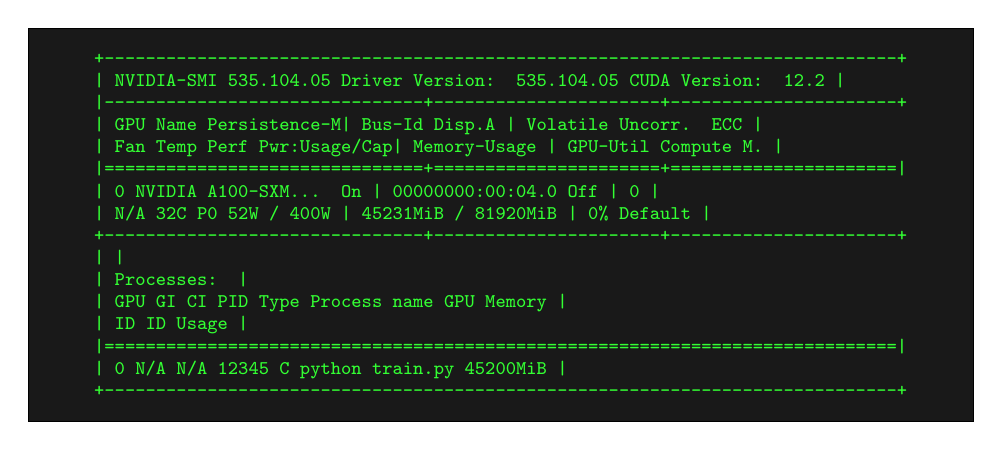
\begin{tikzpicture}[scale=0.9]
    % nvidia-smi 输出示意
    \node[draw, rectangle, fill=black!90, text=green!80, font=\ttfamily\scriptsize, 
          align=left, minimum width=12cm, minimum height=5cm] at (0, 0) {
+-----------------------------------------------------------------------------+\\
| NVIDIA-SMI 535.104.05   Driver Version: 535.104.05   CUDA Version: 12.2     |\\
|-------------------------------+----------------------+----------------------+\\
| GPU  Name        Persistence-M| Bus-Id        Disp.A | Volatile Uncorr. ECC |\\
| Fan  Temp  Perf  Pwr:Usage/Cap|         Memory-Usage | GPU-Util  Compute M. |\\
|===============================+======================+======================|\\
|   0  NVIDIA A100-SXM...  On   | 00000000:00:04.0 Off |                    0 |\\
| N/A   32C    P0    52W / 400W |  45231MiB / 81920MiB |      0\%      Default |\\
+-------------------------------+----------------------+----------------------+\\
|                                                                             |\\
| Processes:                                                                  |\\
|  GPU   GI   CI        PID   Type   Process name                  GPU Memory |\\
|        ID   ID                                                   Usage      |\\
|=============================================================================|\\
|    0   N/A  N/A     12345      C   python train.py                45200MiB |\\
+-----------------------------------------------------------------------------+
    };
\end{tikzpicture}
\caption{\texttt{nvidia-smi}输出示例：显示GPU型号、显存使用、运行中的进程}
\end{figure}

\textbf{文件传输}

\begin{lstlisting}[language=bash, caption=在本地和服务器之间传输文件]
# 从本地上传到服务器
scp local_file.py zhangsan@server:/home/zhangsan/project/

# 从服务器下载到本地
scp zhangsan@server:/home/zhangsan/results.csv ./

# 上传整个文件夹（-r 递归）
scp -r ./my_project zhangsan@server:/home/zhangsan/

# 如果配置了SSH config，可以用别名
scp local_file.py lab:/home/zhangsan/project/
\end{lstlisting}

% ------------------------------------------------------------------------------------
\subsection{Git版本控制}
% ------------------------------------------------------------------------------------

Git是代码版本管理的标准工具。即使只有你一个人写代码，也强烈建议用Git。

\paragraph{为什么要用Git？}

\begin{itemize}
    \item 记录每次修改，可以随时回退
    \item 不用担心改坏代码（改坏了就回退）
    \item 方便在多台机器（本地、服务器）之间同步代码
    \item 方便与他人协作
\end{itemize}

\paragraph{Git基本工作流程}

\begin{figure}[h]
\centering
\begin{tikzpicture}[>=stealth, scale=0.85,
    box/.style={draw, rounded corners, minimum width=2.2cm, minimum height=1cm, align=center}]
    
    % 三个区域
    \node[box, fill=blue!20] (work) at (0, 0) {工作目录\\Working};
    \node[box, fill=green!20] (stage) at (5, 0) {暂存区\\Staging};
    \node[box, fill=orange!20] (repo) at (10, 0) {本地仓库\\Repository};
    \node[box, fill=purple!20] (remote) at (10, -3) {远程仓库\\GitHub/GitLab};
    
    % 箭头
    \draw[->, thick] (work) -- node[above, font=\small] {\texttt{git add}} (stage);
    \draw[->, thick] (stage) -- node[above, font=\small] {\texttt{git commit}} (repo);
    \draw[->, thick] (repo) -- node[right, font=\small] {\texttt{git push}} (remote);
    \draw[->, thick] (remote) -- node[left, font=\small] {\texttt{git pull}} ++(-5, 0) -- (work);
    
\end{tikzpicture}
\caption{Git工作流程}
\end{figure}

\textbf{常用Git命令}

\begin{lstlisting}[language=bash, caption=Git常用命令]
# === 初始化 ===
git init                    # 在当前目录创建Git仓库
git clone <url>             # 克隆远程仓库

# === 日常使用 ===
git status                  # 查看当前状态（哪些文件改了）
git add .                   # 把所有修改添加到暂存区
git add train.py            # 只添加特定文件
git commit -m "描述信息"     # 提交，写清楚这次改了什么

# === 与远程同步 ===
git pull                    # 从远程拉取最新代码
git push                    # 把本地提交推送到远程

# === 查看历史 ===
git log --oneline           # 查看提交历史（简洁版）
git diff                    # 查看未暂存的修改
git diff --staged           # 查看已暂存的修改

# === 分支（进阶） ===
git branch                  # 查看分支
git checkout -b new_feature # 创建并切换到新分支
git merge new_feature       # 合并分支
\end{lstlisting}

\textbf{典型工作流程示例}

\begin{lstlisting}[language=bash, caption=一次完整的Git工作流程]
# 1. 开始工作前，先拉取最新代码
git pull

# 2. 写代码、做实验...

# 3. 查看改了哪些文件
git status

# 4. 添加修改
git add .

# 5. 提交，写清楚改了什么
git commit -m "增加学习率warmup功能"

# 6. 推送到远程（比如GitHub）
git push

# 现在你的代码就安全地保存在远程了！
\end{lstlisting}

\paragraph{.gitignore文件}

有些文件不应该加入Git（比如数据集、模型权重、临时文件）：

\begin{lstlisting}[language=bash, caption=.gitignore示例]
# .gitignore 文件内容

# 数据和模型（太大了）
data/
checkpoints/
*.pt
*.bin

# Python临时文件
__pycache__/
*.pyc
.ipynb_checkpoints/

# 环境和配置
.env
wandb/
outputs/

# 系统文件
.DS_Store
*.log
\end{lstlisting}

% ------------------------------------------------------------------------------------
\subsection{Python环境管理：Conda}
% ------------------------------------------------------------------------------------

服务器上可能有多个用户、多个项目，每个项目需要的Python版本和库可能不同。\textbf{Conda}帮你管理独立的Python环境。

\paragraph{为什么要用虚拟环境？}

\begin{itemize}
    \item 不同项目可能需要不同版本的PyTorch
    \item 避免库版本冲突
    \item 不会污染系统Python
    \item 环境出问题了可以直接删掉重建
\end{itemize}

\textbf{Conda基本命令}

\begin{lstlisting}[language=bash, caption=Conda环境管理]
# === 创建环境 ===
conda create -n myenv python=3.10   # 创建名为myenv的环境，Python 3.10
conda activate myenv                 # 激活环境
conda deactivate                     # 退出环境

# === 查看环境 ===
conda env list                       # 列出所有环境
conda list                           # 列出当前环境的所有包

# === 安装包 ===
conda install numpy pandas           # 用conda安装
pip install torch transformers       # 用pip安装（conda没有的包）

# === 删除环境 ===
conda remove -n myenv --all          # 删除整个环境

# === 导出/导入环境 ===
conda env export > environment.yml   # 导出环境配置
conda env create -f environment.yml  # 从配置文件创建环境
\end{lstlisting}

\textbf{典型深度学习环境配置}

\begin{lstlisting}[language=bash, caption=配置一个深度学习环境]
# 1. 创建新环境
conda create -n llm python=3.10
conda activate llm

# 2. 安装PyTorch（去官网查对应CUDA版本的命令）
# https://pytorch.org/get-started/locally/
pip install torch torchvision torchaudio --index-url https://download.pytorch.org/whl/cu118

# 3. 安装常用库
pip install transformers datasets accelerate
pip install wandb tensorboard
pip install jupyter ipython

# 4. 验证安装
python -c "import torch; print(torch.cuda.is_available())"
# 应该输出 True
\end{lstlisting}

% ------------------------------------------------------------------------------------
\subsection{CUDA与PyTorch版本：公用服务器的大坑}
% ------------------------------------------------------------------------------------

\marginnote{这一节是很多新手踩的最大坑：不理解CUDA版本、PyTorch版本、驱动版本之间的关系，随意升级，结果把组里老代码全搞挂了。}

在公用服务器上，\textbf{版本管理}是一个非常重要但经常被忽视的问题。理解下面这些概念，能帮你避免"一改配置全组遭殃"的惨剧。

\paragraph{三个版本的区别}

\begin{table}[h]
\centering
\small
\renewcommand{\arraystretch}{1.4}
\begin{tabular}{l|l|l|l}
\toprule
\textbf{名称} & \textbf{是什么} & \textbf{谁负责安装} & \textbf{能否随意改} \\
\midrule
\textbf{NVIDIA驱动} & GPU的底层驱动 & 系统管理员 & \textcolor{red}{绝对不能！} \\
\textbf{CUDA Toolkit} & GPU编程工具包 & 系统或用户 & 谨慎（见下文） \\
\textbf{PyTorch CUDA版本} & PyTorch编译时用的CUDA & pip安装时选择 & 可以，但要匹配 \\
\bottomrule
\end{tabular}
\caption{三种"CUDA版本"的区别}
\end{table}

\begin{keyidea}[版本兼容的关键原则]
\begin{itemize}
    \item \textbf{驱动版本} $\geq$ \textbf{CUDA Toolkit版本}（向下兼容）
    \item \textbf{PyTorch CUDA版本}必须与系统CUDA Toolkit匹配
    \item 同一台机器上，\textbf{驱动只有一个}，但可以有多个CUDA Toolkit版本
\end{itemize}
\end{keyidea}

\paragraph{如何查看版本}

\begin{lstlisting}[language=bash, caption=查看各种CUDA相关版本]
# 1. 查看NVIDIA驱动版本（nvidia-smi右上角）
nvidia-smi
# 输出: Driver Version: 535.104.05   CUDA Version: 12.2
#                                     ^^^^^^^^^^^^
#                        注意：这是驱动支持的最高CUDA版本，不是系统安装的CUDA

# 2. 查看系统安装的CUDA Toolkit版本
nvcc --version
# 输出: Cuda compilation tools, release 11.8, V11.8.89

# 3. 查看PyTorch使用的CUDA版本
python -c "import torch; print(torch.version.cuda)"
# 输出: 11.8

# 4. 验证PyTorch能否使用GPU
python -c "import torch; print(torch.cuda.is_available())"
# 输出: True  (如果是False，说明版本不匹配！)
\end{lstlisting}

\begin{remark}
\texttt{nvidia-smi}显示的"CUDA Version"容易让人误解。那是\textbf{驱动支持的最高CUDA版本}，不是你实际安装的CUDA版本。实际版本要用\texttt{nvcc --version}查看。
\end{remark}

\paragraph{什么是 \texttt{cuda:0}？}

当你写 \texttt{.to("cuda:0")} 时，\texttt{cuda:0}表示\textbf{第0号GPU}。

\begin{lstlisting}[language=Python, caption=GPU设备管理]
import torch

# 查看有几张GPU
print(torch.cuda.device_count())  # 比如输出 4，表示有4张卡

# 查看当前默认设备
print(torch.cuda.current_device())  # 通常是 0

# 把张量放到指定GPU
x = torch.randn(1000, 1000)
x = x.to("cuda:0")   # 放到第0张卡
x = x.to("cuda:1")   # 放到第1张卡
x = x.cuda()         # 等价于 .to("cuda:0")

# 指定默认GPU
torch.cuda.set_device(1)  # 之后.cuda()默认用第1张卡
\end{lstlisting}

\paragraph{使用 \texttt{CUDA\_VISIBLE\_DEVICES} 控制可见GPU}

在公用服务器上，你通常不能独占所有GPU。用环境变量控制你的程序能看到哪些卡：

\begin{lstlisting}[language=bash, caption=控制可见GPU]
# 只用第2张卡（编号从0开始）
CUDA_VISIBLE_DEVICES=2 python train.py

# 用第0和第3张卡
CUDA_VISIBLE_DEVICES=0,3 python train.py

# 此时在Python里：
# - torch.cuda.device_count() 返回 2
# - "cuda:0" 对应物理上的第0张卡
# - "cuda:1" 对应物理上的第3张卡

# 完全不用GPU（强制CPU）
CUDA_VISIBLE_DEVICES="" python train.py
\end{lstlisting}

\begin{warning}
\textbf{公用服务器的生存法则}：
\begin{enumerate}
    \item \textbf{永远不要升级系统的CUDA或驱动}——这会影响所有用户！
    \item \textbf{用Conda管理自己的PyTorch版本}——每个环境独立，不影响别人
    \item \textbf{用 \texttt{CUDA\_VISIBLE\_DEVICES} 指定GPU}——避免抢占别人正在用的卡
    \item \textbf{跑之前先 \texttt{nvidia-smi} 看一眼}——确认哪些卡空闲
\end{enumerate}
\end{warning}

\paragraph{版本不匹配的常见报错}

\begin{table}[h]
\centering
\small
\renewcommand{\arraystretch}{1.4}
\begin{tabular}{p{7cm}|p{6cm}}
\toprule
\textbf{报错信息} & \textbf{可能原因} \\
\midrule
\texttt{CUDA error: no kernel image is available} & PyTorch的CUDA版本与GPU架构不匹配 \\
\texttt{torch.cuda.is\_available() = False} & PyTorch没装CUDA版本，或CUDA版本不匹配 \\
\texttt{CUDA out of memory} & 显存不够，或别人在用这张卡 \\
\texttt{RuntimeError: CUDA unknown error} & 驱动问题，尝试重启或联系管理员 \\
\bottomrule
\end{tabular}
\caption{常见CUDA报错与原因}
\end{table}

\paragraph{安装正确版本的PyTorch}

去 \url{https://pytorch.org/get-started/locally/} 选择对应你系统CUDA版本的安装命令：

\begin{lstlisting}[language=bash, caption=根据CUDA版本安装PyTorch]
# 如果系统CUDA是11.8
pip install torch torchvision torchaudio --index-url https://download.pytorch.org/whl/cu118

# 如果系统CUDA是12.1
pip install torch torchvision torchaudio --index-url https://download.pytorch.org/whl/cu121

# CPU版本（没有GPU或想强制用CPU）
pip install torch torchvision torchaudio --index-url https://download.pytorch.org/whl/cpu
\end{lstlisting}

\begin{example}[一个典型的"版本地狱"场景]
\textbf{场景}：师兄的代码在服务器上跑得好好的。你为了跑一个新论文的代码，把系统CUDA从11.8升级到12.2。

\textbf{结果}：
\begin{itemize}
    \item 师兄的PyTorch是cu118版本，现在\texttt{torch.cuda.is\_available()}返回False
    \item 师姐用的TensorFlow也挂了
    \item 导师问为什么大家的实验都跑不了了……
\end{itemize}

\textbf{正确做法}：
\begin{itemize}
    \item 不改系统CUDA，用Conda创建新环境
    \item 在新环境里装cu118版本的PyTorch（向下兼容没问题）
    \item 或者联系管理员，在不影响现有环境的情况下添加新CUDA版本
\end{itemize}
\end{example}

% ------------------------------------------------------------------------------------
\subsection{后台运行：Screen和Tmux}
% ------------------------------------------------------------------------------------

SSH断开后，正在运行的程序会被终止。用\texttt{screen}或\texttt{tmux}可以让程序在后台持续运行。

\textbf{Screen基本用法}

\begin{lstlisting}[language=bash, caption=Screen使用方法]
# 创建新的screen会话
screen -S train          # 创建名为train的会话

# 在screen里运行训练
python train.py

# 断开screen（程序继续运行）
# 按 Ctrl+A，然后按 D

# 重新连接
screen -r train          # 连接到train会话

# 查看所有会话
screen -ls

# 结束会话
exit                     # 在screen里输入exit
# 或者 screen -X -S train quit
\end{lstlisting}

\paragraph{Tmux基本用法}

Tmux功能更强大，推荐使用：

\begin{lstlisting}[language=bash, caption=Tmux使用方法]
# 创建新会话
tmux new -s train

# 断开（detach）
# 按 Ctrl+B，然后按 D

# 重新连接
tmux attach -t train
# 或简写
tmux a -t train

# 查看所有会话
tmux ls

# 结束会话
tmux kill-session -t train
\end{lstlisting}

\begin{figure}[h]
\centering
\begin{tikzpicture}[>=stealth, scale=0.85]

    % 服务器框
    \node[draw, rectangle, fill=blue!10,
          minimum width=10cm, minimum height=4cm] (server) at (0, 0) {};
    \node[above] at (0, 2.2) {服务器};

    % Tmux 会话
\node[
    draw,
    rectangle,
    fill=green!20,
    minimum width=4cm,
    minimum height=1.5cm,
    align=center
] (tmux1) at (-2, 0.5)
    {\texttt{tmux: train}\\\texttt{python train.py}};

\node[
    draw,
    rectangle,
    fill=orange!20,
    minimum width=4cm,
    minimum height=1.5cm,
    align=center
] (tmux2) at (-2, -1.5)
    {\texttt{tmux: eval}\\\texttt{python eval.py}};


    % 用户
    \node[draw, circle, fill=yellow!30] (user) at (6, 0) {你};

    % SSH 连线
    \draw[<->, thick] (user) -- node[above] {SSH} (2, 0);

    % 注释
    \node[right, font=\small, gray] at (7, 1) {SSH断开后};
    \node[right, font=\small, gray] at (7, 0.5) {tmux里的程序};
    \node[right, font=\small, gray] at (7, 0) {继续运行};

\end{tikzpicture}
\caption{Tmux让程序在后台持续运行}
\end{figure}


% ------------------------------------------------------------------------------------
\subsection{集群任务调度：SLURM}
% ------------------------------------------------------------------------------------

如果你使用学校的计算集群（HPC），通常需要通过\textbf{SLURM}提交任务。SLURM会把你的任务排队，等有空闲GPU时自动运行。

\paragraph{SLURM基本概念}

\begin{itemize}
    \item \textbf{节点（Node）}：一台物理服务器
    \item \textbf{分区（Partition）}：一组节点，比如gpu分区、cpu分区
    \item \textbf{作业（Job）}：你提交的任务
    \item \textbf{脚本（Script）}：描述任务需要什么资源、运行什么命令
\end{itemize}

\textbf{查看集群状态}

\begin{lstlisting}[language=bash, caption=SLURM常用查询命令]
# 查看所有分区和节点状态
sinfo

# 查看队列中的作业
squeue

# 只看自己的作业
squeue -u $USER

# 查看作业详细信息
scontrol show job <job_id>

# 查看历史作业
sacct -u $USER --starttime=2024-01-01
\end{lstlisting}

\textbf{编写SLURM脚本}

\begin{lstlisting}[language=bash, caption=SLURM作业脚本示例（train.slurm）]
#!/bin/bash
#SBATCH --job-name=llm_train        # 作业名称
#SBATCH --partition=gpu             # 分区（队列）名称
#SBATCH --nodes=1                   # 节点数
#SBATCH --ntasks-per-node=1         # 每节点任务数
#SBATCH --cpus-per-task=8           # 每任务CPU核数
#SBATCH --gres=gpu:4                # GPU数量
#SBATCH --mem=64G                   # 内存
#SBATCH --time=24:00:00             # 最大运行时间
#SBATCH --output=logs/%j.out        # 标准输出文件（%j是作业ID）
#SBATCH --error=logs/%j.err         # 错误输出文件

# 加载环境
source ~/.bashrc
conda activate llm

# 进入工作目录
cd /home/zhangsan/project

# 运行训练
python train.py \
    --model_name llama-7b \
    --batch_size 4 \
    --learning_rate 2e-5 \
    --num_epochs 3
\end{lstlisting}

\textbf{提交和管理作业}

\begin{lstlisting}[language=bash, caption=提交和管理SLURM作业]
# 提交作业
sbatch train.slurm
# 返回：Submitted batch job 12345

# 查看作业状态
squeue -u $USER
# JOBID  PARTITION  NAME       USER      ST  TIME  NODES  NODELIST
# 12345  gpu        llm_train  zhangsan  R   1:23  1      gpu-node-01

# 取消作业
scancel 12345

# 取消自己的所有作业
scancel -u $USER
\end{lstlisting}

\paragraph{交互式调试}

有时候需要交互式地调试代码，可以申请一个交互式会话：

\begin{lstlisting}[language=bash, caption=申请交互式GPU会话]
# 申请1张GPU，2小时
srun --partition=gpu --gres=gpu:1 --time=2:00:00 --pty bash

# 现在你在一个有GPU的节点上了
nvidia-smi          # 可以看到GPU
python train.py     # 可以直接运行代码

# 退出交互式会话
exit
\end{lstlisting}

\textbf{多GPU训练脚本示例}

\begin{lstlisting}[language=bash, caption=多GPU分布式训练脚本]
#!/bin/bash
#SBATCH --job-name=llm_ddp
#SBATCH --partition=gpu
#SBATCH --nodes=2                   # 2个节点
#SBATCH --ntasks-per-node=4         # 每节点4个任务（对应4张GPU）
#SBATCH --gres=gpu:4                # 每节点4张GPU
#SBATCH --cpus-per-task=4
#SBATCH --mem=128G
#SBATCH --time=48:00:00
#SBATCH --output=logs/%j.out

source ~/.bashrc
conda activate llm

# 设置分布式训练环境变量
export MASTER_ADDR=$(scontrol show hostnames $SLURM_JOB_NODELIST | head -n 1)
export MASTER_PORT=29500
export WORLD_SIZE=$SLURM_NTASKS

# 使用torchrun启动分布式训练
srun torchrun \
    --nnodes=$SLURM_NNODES \
    --nproc_per_node=4 \
    --rdzv_id=$SLURM_JOB_ID \
    --rdzv_backend=c10d \
    --rdzv_endpoint=$MASTER_ADDR:$MASTER_PORT \
    train.py \
    --batch_size 8 \
    --gradient_accumulation_steps 4
\end{lstlisting}

% ------------------------------------------------------------------------------------
\subsection{实用技巧汇总}
% ------------------------------------------------------------------------------------

\textbf{训练监控}

\begin{lstlisting}[language=bash, caption=监控训练过程]
# 实时查看训练日志
tail -f logs/12345.out

# 实时监控GPU
watch -n 1 nvidia-smi

# 使用wandb或tensorboard可视化
# 在训练代码中集成wandb
tensorboard --logdir=./runs --port=6006

# 如果在服务器上运行tensorboard，需要端口转发
# 在本地运行：
ssh -L 6006:localhost:6006 lab
# 然后在本地浏览器打开 http://localhost:6006
\end{lstlisting}

\paragraph{常见问题排查}

\begin{table}[h]
\centering
\small
\renewcommand{\arraystretch}{1.4}
\begin{tabular}{l|l}
\toprule
\textbf{问题} & \textbf{解决方法} \\
\midrule
CUDA out of memory & 减小batch size，用梯度累积 \\
SSH连接断开程序终止 & 用tmux或screen \\
找不到GPU & 检查\texttt{CUDA\_VISIBLE\_DEVICES}环境变量 \\
权限不够 & 检查文件权限，用\texttt{chmod} \\
磁盘空间不足 & \texttt{du -sh *}找大文件，清理checkpoint \\
作业一直排队 & \texttt{sinfo}看资源，考虑换分区或减少资源请求 \\
\bottomrule
\end{tabular}
\caption{常见问题与解决方法}
\end{table}

\textbf{一个完整的实验流程}

\begin{lstlisting}[language=bash, caption=从零开始的完整实验流程]
# === 1. 连接服务器 ===
ssh lab

# === 2. 创建项目目录 ===
mkdir -p ~/projects/my_llm_exp
cd ~/projects/my_llm_exp

# === 3. 克隆代码 ===
git clone https://github.com/yourname/llm-finetune.git
cd llm-finetune

# === 4. 创建环境 ===
conda create -n myexp python=3.10
conda activate myexp
pip install -r requirements.txt

# === 5. 准备数据 ===
mkdir -p data
# 上传或下载数据到 data/ 目录

# === 6. 测试代码（交互式，小数据） ===
srun --partition=gpu --gres=gpu:1 --time=1:00:00 --pty bash
python train.py --debug --max_samples 100
exit

# === 7. 提交正式训练 ===
mkdir -p logs
sbatch train.slurm

# === 8. 监控训练 ===
squeue -u $USER
tail -f logs/<job_id>.out

# === 9. 训练完成后，下载结果 ===
# 在本地：
scp -r lab:~/projects/my_llm_exp/checkpoints ./
\end{lstlisting}

% ------------------------------------------------------------------------------------
\subsection{推荐的目录结构}
% ------------------------------------------------------------------------------------

一个组织良好的项目目录让你的实验更容易管理：

\begin{lstlisting}[language=bash, caption=推荐的项目目录结构]
my_project/
|-- data/                    # 数据（通常不加入git）
|   |-- train.json
|   |-- eval.json
|
|-- src/                     # 源代码
|   |-- model.py
|   |-- train.py
|   |-- eval.py
|   |-- utils.py
|
|-- configs/                 # 配置文件
|   |-- train_7b.yaml
|   |-- train_13b.yaml
|
|-- scripts/                 # 运行脚本
|   |-- train.slurm
|   |-- eval.slurm
|
|-- checkpoints/             # 模型权重（不加入git）
|-- logs/                    # 日志（不加入git）
|-- outputs/                 # 输出结果
|
|-- requirements.txt         # Python依赖
|-- README.md               # 项目说明
|-- .gitignore              # Git忽略文件
\end{lstlisting}

\begin{remark}
养成良好的习惯：
\begin{itemize}
    \item 代码改动及时commit
    \item 重要实验记录配置和结果
    \item checkpoint定期清理（很占空间）
    \item 给文件和变量起有意义的名字
\end{itemize}

这些习惯会在你做毕设或发论文时帮大忙。
\end{remark}

% ------------------------------------------------------------------------------------
\subsection{常用工具库速览}
% ------------------------------------------------------------------------------------

深度学习生态有大量优秀的开源工具。这里介绍最常用的几类，帮你快速上手。

\subsubsection{Hugging Face生态：Transformers + PEFT + Datasets}

\marginnote{\textbf{Hugging Face}：由法国人Clément Delangue等于2016年创立，最初是一个聊天机器人。2019年开源Transformers库后爆发式增长，如今已成为AI开源社区的``GitHub''，托管超过50万个模型。公司估值超40亿美元。}

Hugging Face是目前最流行的NLP/LLM工具生态，几乎是必学的。

\textbf{Transformers：模型加载与推理}

\begin{lstlisting}[language=Python, caption=使用Transformers加载和使用模型]
from transformers import AutoTokenizer, AutoModelForCausalLM
import torch

# 加载模型和分词器（会自动从Hugging Face下载）
model_name = "meta-llama/Llama-2-7b-hf"  # 或本地路径
tokenizer = AutoTokenizer.from_pretrained(model_name)
model = AutoModelForCausalLM.from_pretrained(
    model_name,
    torch_dtype=torch.float16,  # 半精度节省显存
    device_map="auto"           # 自动分配到GPU
)

# 生成文本
prompt = "人工智能的未来发展方向是"
inputs = tokenizer(prompt, return_tensors="pt").to(model.device)
outputs = model.generate(
    **inputs,
    max_new_tokens=100,
    temperature=0.7,
    do_sample=True
)
print(tokenizer.decode(outputs[0], skip_special_tokens=True))
\end{lstlisting}

\paragraph{PEFT：参数高效微调（LoRA等）}

PEFT（Parameter-Efficient Fine-Tuning）库让你用几行代码就能实现LoRA微调：

\begin{lstlisting}[language=Python, caption=使用PEFT进行LoRA微调]
from transformers import AutoModelForCausalLM, AutoTokenizer, TrainingArguments
from peft import LoraConfig, get_peft_model, TaskType
from trl import SFTTrainer

# 1. 加载基础模型
model = AutoModelForCausalLM.from_pretrained(
    "meta-llama/Llama-2-7b-hf",
    torch_dtype=torch.float16,
    device_map="auto"
)

# 2. 配置LoRA
lora_config = LoraConfig(
    task_type=TaskType.CAUSAL_LM,
    r=8,                        # LoRA秩
    lora_alpha=16,              # 缩放因子
    lora_dropout=0.05,
    target_modules=["q_proj", "v_proj"],  # 对哪些层应用LoRA
)

# 3. 创建PEFT模型
model = get_peft_model(model, lora_config)
model.print_trainable_parameters()
# 输出类似：trainable params: 4,194,304 || all params: 6,742,609,920 || trainable%: 0.0622

# 4. 训练（使用trl的SFTTrainer更方便）
trainer = SFTTrainer(
    model=model,
    train_dataset=dataset,
    args=TrainingArguments(
        output_dir="./output",
        per_device_train_batch_size=4,
        gradient_accumulation_steps=4,
        num_train_epochs=3,
        learning_rate=2e-4,
        fp16=True,
        logging_steps=10,
        save_steps=100,
    ),
)
trainer.train()

# 5. 保存LoRA权重（只保存增量，很小）
model.save_pretrained("./lora_weights")
\end{lstlisting}

\textbf{Datasets：数据加载与处理}

\begin{lstlisting}[language=Python, caption=使用Datasets处理数据]
from datasets import load_dataset, Dataset

# 加载公开数据集
dataset = load_dataset("tatsu-lab/alpaca")  # 指令微调数据

# 加载本地JSON文件
dataset = load_dataset("json", data_files="data/train.json")

# 从Python字典创建
data = {
    "instruction": ["写一首诗", "翻译成英文"],
    "input": ["关于春天", "你好世界"],
    "output": ["春风拂面...", "Hello World"]
}
dataset = Dataset.from_dict(data)

# 数据预处理
def preprocess(example):
    prompt = f"### 指令:\n{example['instruction']}\n### 回答:\n"
    return {"text": prompt + example["output"]}

dataset = dataset.map(preprocess)

# 划分训练集和验证集
dataset = dataset.train_test_split(test_size=0.1)
\end{lstlisting}

\begin{table}[h]
\centering
\small
\renewcommand{\arraystretch}{1.3}
\begin{tabular}{l|l|l}
\toprule
\textbf{库} & \textbf{功能} & \textbf{安装} \\
\midrule
transformers & 模型加载、推理、训练 & \texttt{pip install transformers} \\
peft & LoRA、QLoRA等高效微调 & \texttt{pip install peft} \\
datasets & 数据集加载与处理 & \texttt{pip install datasets} \\
accelerate & 分布式训练、混合精度 & \texttt{pip install accelerate} \\
trl & RLHF、SFT训练器 & \texttt{pip install trl} \\
bitsandbytes & 4/8-bit量化 & \texttt{pip install bitsandbytes} \\
\bottomrule
\end{tabular}
\caption{Hugging Face生态常用库}
\end{table}

\subsubsection{量化推理：让大模型在小显卡上跑}

显存不够时，量化是最直接的解决方案。

\textbf{BitsAndBytes：4-bit/8-bit量化}

\begin{lstlisting}[language=Python, caption=4-bit量化加载模型]
from transformers import AutoModelForCausalLM, AutoTokenizer, BitsAndBytesConfig

# 配置4-bit量化
bnb_config = BitsAndBytesConfig(
    load_in_4bit=True,                    # 4-bit加载
    bnb_4bit_quant_type="nf4",           # NormalFloat4量化
    bnb_4bit_compute_dtype=torch.float16, # 计算时用FP16
    bnb_4bit_use_double_quant=True,      # 二次量化，进一步压缩
)

# 加载量化模型
model = AutoModelForCausalLM.from_pretrained(
    "meta-llama/Llama-2-7b-hf",
    quantization_config=bnb_config,
    device_map="auto"
)
# 原本需要14GB显存，现在只需要约4GB！
\end{lstlisting}

\paragraph{QLoRA：量化 + LoRA}

QLoRA结合了量化和LoRA，可以在单张消费级显卡上微调大模型：

\begin{lstlisting}[language=Python, caption=QLoRA微调]
from peft import prepare_model_for_kbit_training

# 1. 加载4-bit量化模型
model = AutoModelForCausalLM.from_pretrained(
    "meta-llama/Llama-2-7b-hf",
    quantization_config=bnb_config,
    device_map="auto"
)

# 2. 准备模型进行k-bit训练
model = prepare_model_for_kbit_training(model)

# 3. 添加LoRA
model = get_peft_model(model, lora_config)

# 现在可以在RTX 3080 (10GB) 上微调7B模型了！
\end{lstlisting}

\textbf{GPTQ/AWQ：更高效的量化}

\begin{lstlisting}[language=Python, caption=加载GPTQ量化模型]
from transformers import AutoModelForCausalLM

# GPTQ量化模型（需要预先量化好的权重）
model = AutoModelForCausalLM.from_pretrained(
    "TheBloke/Llama-2-7B-GPTQ",  # 社区量化的模型
    device_map="auto"
)
\end{lstlisting}

\begin{table}[h]
\centering
\small
\renewcommand{\arraystretch}{1.3}
\begin{tabular}{l|c|c|l}
\toprule
\textbf{量化方法} & \textbf{精度} & \textbf{7B模型显存} & \textbf{特点} \\
\midrule
无量化 (FP16) & 高 & 14 GB & 基准 \\
BitsAndBytes 8-bit & 较高 & 8 GB & 简单易用 \\
BitsAndBytes 4-bit & 中等 & 4-5 GB & 配合LoRA微调 \\
GPTQ 4-bit & 中等 & 4 GB & 推理快，需预量化 \\
AWQ 4-bit & 中等 & 4 GB & 推理更快 \\
\bottomrule
\end{tabular}
\caption{常见量化方法对比}
\end{table}

\subsubsection{高效推理框架}

当你需要部署模型提供服务时，这些框架能大幅提升吞吐量。

\paragraph{vLLM：高吞吐量推理}

vLLM使用PagedAttention技术，显著提升推理效率：

\begin{lstlisting}[language=Python, caption=使用vLLM进行高效推理]
from vllm import LLM, SamplingParams

# 加载模型
llm = LLM(
    model="meta-llama/Llama-2-7b-hf",
    tensor_parallel_size=1,  # GPU数量
    dtype="float16"
)

# 配置采样参数
sampling_params = SamplingParams(
    temperature=0.7,
    top_p=0.9,
    max_tokens=256
)

# 批量推理（vLLM会自动优化批处理）
prompts = [
    "北京是中国的",
    "机器学习的核心思想是",
    "今天天气很好，我想"
]
outputs = llm.generate(prompts, sampling_params)

for output in outputs:
    print(output.outputs[0].text)
\end{lstlisting}

\textbf{启动vLLM API服务}

\begin{lstlisting}[language=bash, caption=启动vLLM服务器]
# 启动OpenAI兼容的API服务
python -m vllm.entrypoints.openai.api_server \
    --model meta-llama/Llama-2-7b-hf \
    --port 8000

# 然后可以用OpenAI的客户端调用
# curl http://localhost:8000/v1/completions ...
\end{lstlisting}

\paragraph{其他推理框架}

\begin{table}[h]
\centering
\small
\renewcommand{\arraystretch}{1.3}
\begin{tabular}{l|l|l}
\toprule
\textbf{框架} & \textbf{特点} & \textbf{适用场景} \\
\midrule
vLLM & PagedAttention，高吞吐 & 生产部署 \\
Text Generation Inference & Hugging Face官方 & 容器化部署 \\
llama.cpp & CPU/低端GPU推理 & 本地运行、边缘设备 \\
Ollama & 一键运行本地模型 & 个人使用、快速体验 \\
\bottomrule
\end{tabular}
\caption{常见推理框架对比}
\end{table}

\subsubsection{LangChain：构建LLM应用}

LangChain是构建LLM应用的流行框架，提供了链式调用、RAG、Agent等功能。

\textbf{基本使用}

\begin{lstlisting}[language=Python, caption=LangChain基本使用]
from langchain_openai import ChatOpenAI
from langchain_core.prompts import ChatPromptTemplate
from langchain_core.output_parsers import StrOutputParser

# 1. 创建模型（可以用OpenAI或本地模型）
llm = ChatOpenAI(
    model="gpt-3.5-turbo",
    temperature=0.7
)

# 2. 创建提示模板
prompt = ChatPromptTemplate.from_messages([
    ("system", "你是一个专业的{role}。"),
    ("user", "{question}")
])

# 3. 创建链（Chain）
chain = prompt | llm | StrOutputParser()

# 4. 运行
response = chain.invoke({
    "role": "Python程序员",
    "question": "如何读取CSV文件？"
})
print(response)
\end{lstlisting}

\paragraph{RAG：检索增强生成}

RAG让模型能够基于你的文档回答问题：

\begin{lstlisting}[language=Python, caption=使用LangChain构建RAG系统]
from langchain_community.document_loaders import PyPDFLoader
from langchain.text_splitter import RecursiveCharacterTextSplitter
from langchain_community.vectorstores import FAISS
from langchain_openai import OpenAIEmbeddings
from langchain.chains import RetrievalQA

# 1. 加载文档
loader = PyPDFLoader("paper.pdf")
documents = loader.load()

# 2. 切分文档
text_splitter = RecursiveCharacterTextSplitter(
    chunk_size=1000,
    chunk_overlap=200
)
splits = text_splitter.split_documents(documents)

# 3. 创建向量存储
embeddings = OpenAIEmbeddings()
vectorstore = FAISS.from_documents(splits, embeddings)

# 4. 创建检索QA链
qa_chain = RetrievalQA.from_chain_type(
    llm=ChatOpenAI(model="gpt-3.5-turbo"),
    chain_type="stuff",
    retriever=vectorstore.as_retriever(search_kwargs={"k": 3})
)

# 5. 提问
answer = qa_chain.invoke("这篇论文的主要贡献是什么？")
print(answer)
\end{lstlisting}

\begin{figure}[h]
\centering
\begin{tikzpicture}[>=stealth, scale=0.8,
    box/.style={draw, rounded corners, minimum width=2cm, minimum height=1cm, align=center, font=\small}]
    
    % RAG流程
    \node[box, fill=blue!20] (query) at (0, 0) {用户问题};
    \node[box, fill=green!20] (embed) at (3, 0) {向量化};
    \node[box, fill=orange!20] (search) at (6, 0) {检索相关\\文档};
    \node[box, fill=purple!20] (llm) at (9, 0) {LLM生成\\回答};
    \node[box, fill=red!20] (answer) at (12, 0) {最终答案};
    
    % 向量数据库
    \node[box, fill=yellow!20] (db) at (6, -2.5) {向量数据库\\(文档切片)};
    
    % 箭头
    \draw[->, thick] (query) -- (embed);
    \draw[->, thick] (embed) -- (search);
    \draw[->, thick] (search) -- (llm);
    \draw[->, thick] (llm) -- (answer);
    \draw[->, thick] (search) -- (db);
    \draw[->, thick] (db) -- (search);
    
\end{tikzpicture}
\caption{RAG（检索增强生成）流程}
\end{figure}

\paragraph{Agent：让LLM使用工具}

Agent可以让LLM调用外部工具（搜索、计算器、代码执行等）：

\begin{lstlisting}[language=Python, caption=创建简单的Agent]
from langchain_openai import ChatOpenAI
from langchain.agents import tool, AgentExecutor, create_react_agent
from langchain import hub

# 1. 定义工具
@tool
def search_weather(city: str) -> str:
    """查询城市天气"""
    # 实际应该调用天气API
    return f"{city}今天晴，气温25度"

@tool  
def calculate(expression: str) -> str:
    """计算数学表达式"""
    return str(eval(expression))

tools = [search_weather, calculate]

# 2. 创建Agent
llm = ChatOpenAI(model="gpt-4", temperature=0)
prompt = hub.pull("hwchase17/react")  # 使用ReAct提示模板
agent = create_react_agent(llm, tools, prompt)

# 3. 创建执行器
agent_executor = AgentExecutor(
    agent=agent, 
    tools=tools, 
    verbose=True  # 打印推理过程
)

# 4. 运行
response = agent_executor.invoke({
    "input": "北京今天天气怎么样？如果温度乘以2是多少？"
})
print(response["output"])
\end{lstlisting}

\subsubsection{实验追踪：Weights \& Biases}

W\&B（wandb）帮你记录实验、可视化训练曲线、比较不同配置：

\begin{lstlisting}[language=Python, caption=使用W\&B追踪实验]
import wandb

# 1. 初始化（第一次需要登录：wandb login）
wandb.init(
    project="llm-finetune",      # 项目名
    name="lora-r8-lr2e4",        # 本次实验名
    config={                      # 记录超参数
        "model": "llama-7b",
        "lora_r": 8,
        "learning_rate": 2e-4,
        "batch_size": 4,
    }
)

# 2. 在训练循环中记录指标
for epoch in range(num_epochs):
    for batch in dataloader:
        loss = train_step(batch)
        wandb.log({
            "train/loss": loss,
            "train/epoch": epoch
        })
    
    # 验证
    val_loss = evaluate()
    wandb.log({"val/loss": val_loss})

# 3. 结束
wandb.finish()

# 如果使用HuggingFace Trainer，直接设置report_to="wandb"即可
\end{lstlisting}

\begin{figure}[h]
\centering
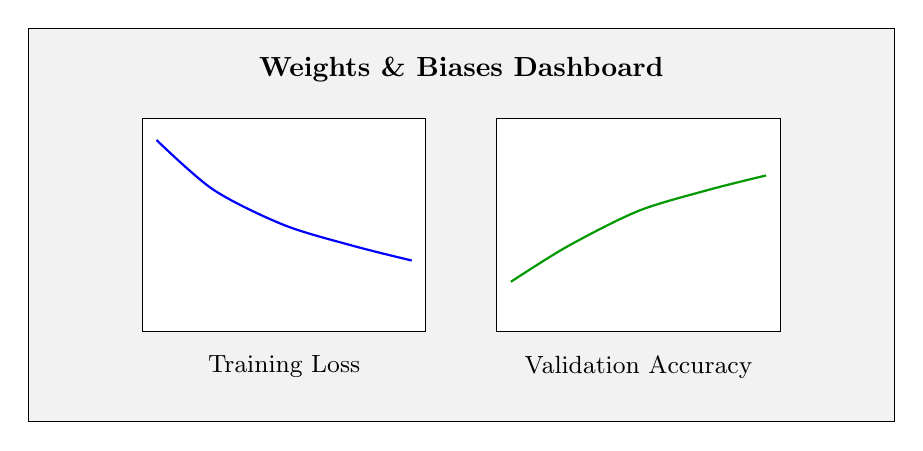
\begin{tikzpicture}[scale=0.9]
    % W&B界面示意
    \node[draw, rectangle, fill=gray!10, minimum width=11cm, minimum height=5cm] at (0, 0) {};
    
    % 图表区域
    \draw[fill=white] (-4.5, -1.5) rectangle (-0.5, 1.5);
    \draw[thick, blue, smooth] plot coordinates {(-4.3, 1.2) (-3.5, 0.5) (-2.5, 0) (-1.5, -0.3) (-0.7, -0.5)};
    \node[font=\small] at (-2.5, -2) {Training Loss};
    
    \draw[fill=white] (0.5, -1.5) rectangle (4.5, 1.5);
    \draw[thick, green!60!black, smooth] plot coordinates {(0.7, -0.8) (1.5, -0.3) (2.5, 0.2) (3.5, 0.5) (4.3, 0.7)};
    \node[font=\small] at (2.5, -2) {Validation Accuracy};
    
    % 标题
    \node[font=\bfseries] at (0, 2.2) {Weights \& Biases Dashboard};
    
\end{tikzpicture}
\caption{W\&B自动生成训练曲线和实验对比}
\end{figure}

\subsubsection{工具库速查表}

\begin{table}[h]
\centering
\small
\renewcommand{\arraystretch}{1.4}
\begin{tabular}{l|l|l}
\toprule
\textbf{任务} & \textbf{推荐工具} & \textbf{一句话说明} \\
\midrule
\multicolumn{3}{c}{\textit{模型训练与微调}} \\
\midrule
加载预训练模型 & Transformers & \texttt{AutoModel.from\_pretrained()} \\
LoRA/QLoRA微调 & PEFT + BitsAndBytes & 低显存微调大模型 \\
分布式训练 & Accelerate / DeepSpeed & 多卡/多机训练 \\
RLHF训练 & TRL & PPO、DPO实现 \\
\midrule
\multicolumn{3}{c}{\textit{推理与部署}} \\
\midrule
高效批量推理 & vLLM & PagedAttention，高吞吐 \\
本地快速体验 & Ollama & \texttt{ollama run llama2} \\
CPU/边缘推理 & llama.cpp & C++实现，无需GPU \\
\midrule
\multicolumn{3}{c}{\textit{应用开发}} \\
\midrule
构建LLM应用 & LangChain & 链式调用、RAG、Agent \\
向量数据库 & FAISS / Chroma & 存储和检索文档向量 \\
\midrule
\multicolumn{3}{c}{\textit{实验管理}} \\
\midrule
实验追踪 & Weights \& Biases & 记录指标、可视化 \\
可视化 & TensorBoard & \texttt{tensorboard --logdir=runs} \\
\bottomrule
\end{tabular}
\caption{常用工具库速查}
\end{table}

\subsubsection{一个完整的微调示例}

把前面的工具组合起来，这是一个完整的LoRA微调脚本：

\begin{lstlisting}[language=Python, caption=完整的LoRA微调脚本]
"""
LLaMA LoRA微调完整示例
运行: python finetune.py
"""
import torch
from datasets import load_dataset
from transformers import (
    AutoModelForCausalLM,
    AutoTokenizer,
    TrainingArguments,
    BitsAndBytesConfig,
)
from peft import LoraConfig, get_peft_model, prepare_model_for_kbit_training
from trl import SFTTrainer
import wandb

# ============ 配置 ============
MODEL_NAME = "meta-llama/Llama-2-7b-hf"
OUTPUT_DIR = "./output"
LORA_R = 8
LORA_ALPHA = 16
LEARNING_RATE = 2e-4
BATCH_SIZE = 4
GRAD_ACCUM = 4
NUM_EPOCHS = 3
MAX_SEQ_LEN = 1024

# ============ 初始化W&B ============
wandb.init(project="llm-finetune", name="lora-alpaca")

# ============ 加载模型（4-bit量化）============
bnb_config = BitsAndBytesConfig(
    load_in_4bit=True,
    bnb_4bit_quant_type="nf4",
    bnb_4bit_compute_dtype=torch.float16,
)

model = AutoModelForCausalLM.from_pretrained(
    MODEL_NAME,
    quantization_config=bnb_config,
    device_map="auto",
)
tokenizer = AutoTokenizer.from_pretrained(MODEL_NAME)
tokenizer.pad_token = tokenizer.eos_token

# ============ 配置LoRA ============
model = prepare_model_for_kbit_training(model)
lora_config = LoraConfig(
    r=LORA_R,
    lora_alpha=LORA_ALPHA,
    lora_dropout=0.05,
    target_modules=["q_proj", "v_proj", "k_proj", "o_proj"],
    task_type="CAUSAL_LM",
)
model = get_peft_model(model, lora_config)
model.print_trainable_parameters()

# ============ 加载数据 ============
dataset = load_dataset("tatsu-lab/alpaca", split="train")

def format_prompt(example):
    if example["input"]:
        text = f"### Instruction:\n{example['instruction']}\n\n### Input:\n{example['input']}\n\n### Response:\n{example['output']}"
    else:
        text = f"### Instruction:\n{example['instruction']}\n\n### Response:\n{example['output']}"
    return {"text": text}

dataset = dataset.map(format_prompt)

# ============ 训练 ============
trainer = SFTTrainer(
    model=model,
    train_dataset=dataset,
    dataset_text_field="text",
    max_seq_length=MAX_SEQ_LEN,
    args=TrainingArguments(
        output_dir=OUTPUT_DIR,
        per_device_train_batch_size=BATCH_SIZE,
        gradient_accumulation_steps=GRAD_ACCUM,
        num_train_epochs=NUM_EPOCHS,
        learning_rate=LEARNING_RATE,
        fp16=True,
        logging_steps=10,
        save_steps=200,
        save_total_limit=3,
        report_to="wandb",
        warmup_ratio=0.03,
    ),
)

trainer.train()

# ============ 保存 ============
model.save_pretrained(f"{OUTPUT_DIR}/lora_weights")
tokenizer.save_pretrained(f"{OUTPUT_DIR}/lora_weights")
wandb.finish()

print("训练完成！")
\end{lstlisting}

\begin{lstlisting}[language=bash, caption=对应的SLURM脚本]
#!/bin/bash
#SBATCH --job-name=lora_finetune
#SBATCH --partition=gpu
#SBATCH --gres=gpu:1
#SBATCH --cpus-per-task=8
#SBATCH --mem=32G
#SBATCH --time=12:00:00
#SBATCH --output=logs/%j.out

source ~/.bashrc
conda activate llm

cd /home/user/project
python finetune.py
\end{lstlisting}

\begin{remark}
工具在快速迭代，API可能会变化。建议：
\begin{itemize}
    \item 遇到问题先看官方文档和GitHub Issues
    \item 记录你使用的库版本（\texttt{pip freeze > requirements.txt}）
    \item 从官方示例代码开始修改，而不是从零写起
\end{itemize}
\end{remark}